% Options for packages loaded elsewhere
\PassOptionsToPackage{unicode}{hyperref}
\PassOptionsToPackage{hyphens}{url}
%
\documentclass[
]{book}
\usepackage{lmodern}
\usepackage{amssymb,amsmath}
\usepackage{ifxetex,ifluatex}
\ifnum 0\ifxetex 1\fi\ifluatex 1\fi=0 % if pdftex
  \usepackage[T1]{fontenc}
  \usepackage[utf8]{inputenc}
  \usepackage{textcomp} % provide euro and other symbols
\else % if luatex or xetex
  \usepackage{unicode-math}
  \defaultfontfeatures{Scale=MatchLowercase}
  \defaultfontfeatures[\rmfamily]{Ligatures=TeX,Scale=1}
\fi
% Use upquote if available, for straight quotes in verbatim environments
\IfFileExists{upquote.sty}{\usepackage{upquote}}{}
\IfFileExists{microtype.sty}{% use microtype if available
  \usepackage[]{microtype}
  \UseMicrotypeSet[protrusion]{basicmath} % disable protrusion for tt fonts
}{}
\makeatletter
\@ifundefined{KOMAClassName}{% if non-KOMA class
  \IfFileExists{parskip.sty}{%
    \usepackage{parskip}
  }{% else
    \setlength{\parindent}{0pt}
    \setlength{\parskip}{6pt plus 2pt minus 1pt}}
}{% if KOMA class
  \KOMAoptions{parskip=half}}
\makeatother
\usepackage{xcolor}
\IfFileExists{xurl.sty}{\usepackage{xurl}}{} % add URL line breaks if available
\IfFileExists{bookmark.sty}{\usepackage{bookmark}}{\usepackage{hyperref}}
\hypersetup{
  pdftitle={MSc Psychology (Conversion) - Experiment Library},
  pdfauthor={Jennifer Mattschey},
  hidelinks,
  pdfcreator={LaTeX via pandoc}}
\urlstyle{same} % disable monospaced font for URLs
\usepackage{longtable,booktabs}
% Correct order of tables after \paragraph or \subparagraph
\usepackage{etoolbox}
\makeatletter
\patchcmd\longtable{\par}{\if@noskipsec\mbox{}\fi\par}{}{}
\makeatother
% Allow footnotes in longtable head/foot
\IfFileExists{footnotehyper.sty}{\usepackage{footnotehyper}}{\usepackage{footnote}}
\makesavenoteenv{longtable}
\usepackage{graphicx,grffile}
\makeatletter
\def\maxwidth{\ifdim\Gin@nat@width>\linewidth\linewidth\else\Gin@nat@width\fi}
\def\maxheight{\ifdim\Gin@nat@height>\textheight\textheight\else\Gin@nat@height\fi}
\makeatother
% Scale images if necessary, so that they will not overflow the page
% margins by default, and it is still possible to overwrite the defaults
% using explicit options in \includegraphics[width, height, ...]{}
\setkeys{Gin}{width=\maxwidth,height=\maxheight,keepaspectratio}
% Set default figure placement to htbp
\makeatletter
\def\fps@figure{htbp}
\makeatother
\setlength{\emergencystretch}{3em} % prevent overfull lines
\providecommand{\tightlist}{%
  \setlength{\itemsep}{0pt}\setlength{\parskip}{0pt}}
\setcounter{secnumdepth}{5}
\usepackage{booktabs}
\usepackage{amsthm}
\makeatletter
\def\thm@space@setup{%
  \thm@preskip=8pt plus 2pt minus 4pt
  \thm@postskip=\thm@preskip
}
\makeatother
\usepackage[]{natbib}
\bibliographystyle{apalike}

\title{MSc Psychology (Conversion) - Experiment Library}
\author{Jennifer Mattschey}
\date{2020-09-14}

\begin{document}
\maketitle

{
\setcounter{tocdepth}{1}
\tableofcontents
}
\hypertarget{psychology-conversion-course-experiment-library}{%
\chapter{Psychology Conversion Course Experiment Library}\label{psychology-conversion-course-experiment-library}}

This collection of experiments was created for the \href{https://www.strath.ac.uk/courses/postgraduatetaught/psychologywithaspecialisationinbusiness}{MSc in Psychology}, an online Psychology conversion course at the University of Strathclyde. The projects aim to provide students with a starting point, from which they can develop their own experiments. Please note that some projects are copyright protected and the files for them are stored in the university network.

Currently, only the section on intelligence tests is affected by these restrictions. If you are a student at the University Strathclyde, please ask your supervisor to send you the files. They will be able to locate them in the conversion course Empirical Project folder on their i-drive.

If you are viewing the PDF or EPUB version, it is worth mentioning that the few gifs that have been embedded will not be displayed. If you come across a reference to a Figure that you cannot see, please refer back to this online version.

\hypertarget{choosing-an-experiment-for-your-research-project}{%
\section{Choosing an Experiment for your Research Project}\label{choosing-an-experiment-for-your-research-project}}

This book will discuss some research paradigms and commonly used types of experiments. Each experiment will be accompanied by a finished experiment file and/or the materials required to create the experiment. We will primarily focus on tasks that run in Open Sesame and questionnaires we can use on Qualtrics.

Online experiments should generally be kept short. As a rough rule of thumb, try to aim for 20 minutes or less. Please keep this mind when you choose which tasks to include in your study. In general, it is better to have a shorter experiment that has been completed by more participants, than to have a longer experiment completed by fewer participants

\hypertarget{how-to-use-the-experiment-library}{%
\section{How to use the Experiment Library}\label{how-to-use-the-experiment-library}}

For each task you will see an Open Sesame file and/or Qualtrics file included. You can download these files and use them to test participants. At the end of this book, you find chapters that explain how to use these files. However, some information on how to adapt experiment files is also provided throughout the book.

\hypertarget{accessibility}{%
\section{Accessibility}\label{accessibility}}

If you look at the top of this page, you will see a menu with several symbols. If you click on the `A', you can adapt the font to your liking and change the colour scheme.

\begin{figure}

{\centering 
\includegraphics[width=0.95\linewidth]{images/accessibility} 

}

\caption{Click on the A to find alternative fonts and colour schemes}\label{fig:Figure0-1}
\end{figure}

It is also possible to search the Experiment Library from this menu and to download the book as epub or PDF. Please note that while the epub and PDF version contain most Figures, these versions do not currently include any Figures in gif format. If you notice a reference to a Figure that is not contained within these versions, it is likely to be a gif that you will be able to view in the online version.

\hypertarget{downloading-files-from-github}{%
\section{Downloading files from GitHub}\label{downloading-files-from-github}}

If you have never used GitHub, it might look a little confusing and the download button can be difficult to find When you click on the link that leads you to the experiment file, you will see something like the picture below. Just press the download button (framed in red) to download the file.

\begin{figure}

{\centering 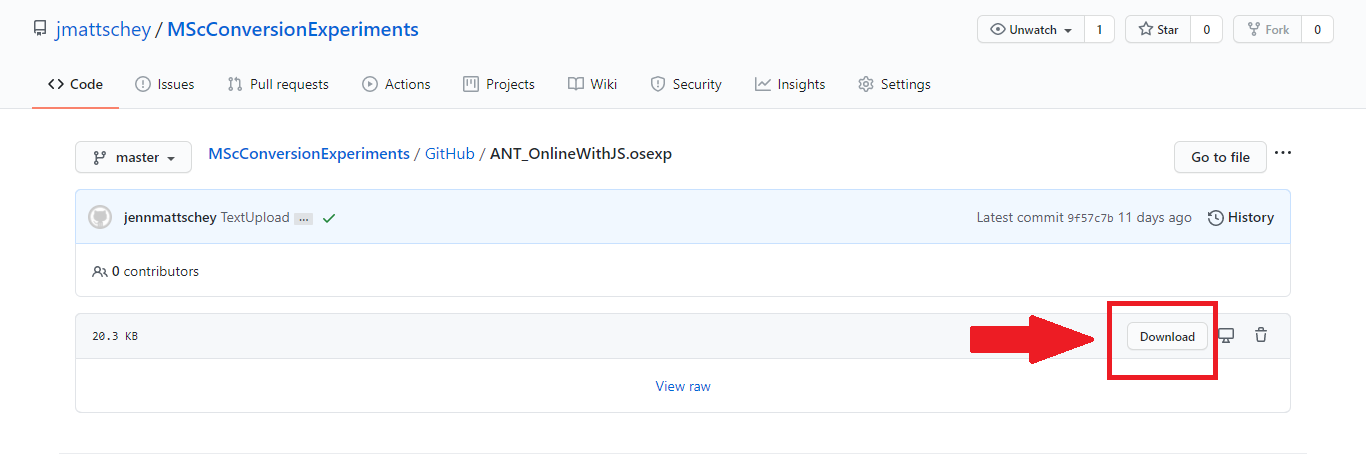
\includegraphics[width=0.95\linewidth]{images/opensesame/download} 

}

\caption{Click the download button to start downloading the experiment.}\label{fig:Figure0-2}
\end{figure}

\hypertarget{other-institutions-and-non-psychology-staff-and-students}{%
\section{Other institutions and non-Psychology staff and students}\label{other-institutions-and-non-psychology-staff-and-students}}

If you are a student or member of staff at the University of Strathclyde, you will have access to all files. However, if you do not have access to the C8983: Empirical Project MyPlace page, you might have to email \href{jennifer.mattschey@strath.ac}{Dr Jennifer Mattschey} to gain access to some of the materials. Please use your Strathclyde email address to do so.

If you are \textbf{not} a Strathclyde student or member of staff, you are still welcome to use these resources. However, some will be password protected due to copyright issues. If you use any of the experiments, please acknowledge the source of the experiment file by citing this Experiment Library.

\hypertarget{adapting-the-experiment-library-for-other-courses}{%
\subsection{Adapting the Experiment Library for other courses}\label{adapting-the-experiment-library-for-other-courses}}

The Experiment Library was created using the bookdown package in R (Xie, 2016, 2020). The copyrighted material is not accessible to anyone who is not employed by or studying at the University of Strathclyde. The Experiment Library itself and openly available files are shared under the \href{https://creativecommons.org/licenses/by-sa/4.0/}{Creative Commons Attribution-ShareAlike 4.0 International (CC BY-SA 4.0) licence}. Please check the license link to check how the code and files can be used and adapted.

\textbf{References}
Xie Y (2020). bookdown: Authoring Books and Technical Documents with R Markdown. R package version 0.20, \url{https://github.com/rstudio/bookdown}.

Xie Y (2016). bookdown: Authoring Books and Technical Documents with R Markdown. Chapman and Hall/CRC, Boca Raton, Florida. ISBN 978-1138700109, \url{https://github.com/rstudio/bookdown}.

\hypertarget{intelligence-tests}{%
\chapter{Intelligence Tests}\label{intelligence-tests}}

The intelligence tests listed in the following are copyright protected and therefore only available to staff and students at the University of Strathclyde.

The tests are suitable to test adults of below average intelligence, average intelligence, and above average intelligence. For children aged 4 to 11 years, the Crichton Vocabulary Scale and Coloured Progressive Matrices are included.

Remember to check if aspects of your experiment design may affect your measures. For example, bilinguals tend to perform worse on verbal intelligence tests than monolinguals but both groups perform equally well on non-verbal intelligence tests. Thus, if you think this may affect the outcome of your findings, you should record whether your participants are bilingual.

\hypertarget{ravens-matrices-for-adults}{%
\section{Raven's Matrices for Adults}\label{ravens-matrices-for-adults}}

Three different sets of Raven's Matrices can be used to test non-verbal intelligence in adults:

\begin{enumerate}
\def\labelenumi{\arabic{enumi}.}
\tightlist
\item
  \textbf{Raven's Progressive Matrices:} 60 matrices that become increasingly difficult
\item
  \textbf{Raven's Progressive Matrices Abbreviated Nine-item Forms:} short versions on Raven's Progressive Matrices, each test only contains nine matrices
\item
  \textbf{Raven's Advanced Progressive Matrices:} contains 48 items in two sets of matrices, and aims to assess non-verbal intelligence of adults and adolescents who can be expected to have above average intelligence
\end{enumerate}

\textbf{How to use the Raven's Progressive Matrices}

To get a full picture of a person's intelligence, the Mill Hill Vocabulary Test (see below) should be administered alongside Raven's Matrices. For children, a Coloured Progressive Matrices and the Crichton Vocabulary Scale should be used instead. If you will be testing adults who would be expected to score below average intelligence, it may be appropriate to use the Coloured Progressive Matrices and Crichton Vocabulary Scale instead. It is best to discuss the choice of test with your supervisor.

\textbf{Formats}

At the moment, the following versions are available for Psychology students at the University of Strathclyde:

Please talk to your supervisor to get the Open Sesame files.

\textbf{Things you will need to know for your Methods section}

If you look at the \textbf{Ravens loop} in Raven's Advanced Progressive Matrices you will notice that the first matrix of Set I is not included in the loop. Instead, the first matrix of Set I is shown as an example for participants.

The 9-Item file contains both Form A and Form B. Participants are expected to complete only one of these, please delete the one you do not want to use. The example shown in the 9-item version is A5 in the in the Standard Matrices.

\hypertarget{shortening-ravens-advanced-progressive-matrices}{%
\subsection{Shortening Raven's Advanced Progressive Matrices}\label{shortening-ravens-advanced-progressive-matrices}}

Raven's Advanced Progressive Matrices consist of two sets of stimuli:

\begin{itemize}
\tightlist
\item
  \textbf{Set I:} 12 Stimuli
\item
  \textbf{Set II:} 36 Stimuli
\end{itemize}

Participants often find it difficult to focus for a long time on online experiments so you may wish to remove a set or some of the stimuli. To do this, open the file in Open Sesame and select the \textbf{``Ravens'' loop}. You will see a table that lists each stimulus and the correct response. Simply highlight the items that you want to remove, right-click on them, and choose ``delete row.''

\begin{figure}

{\centering 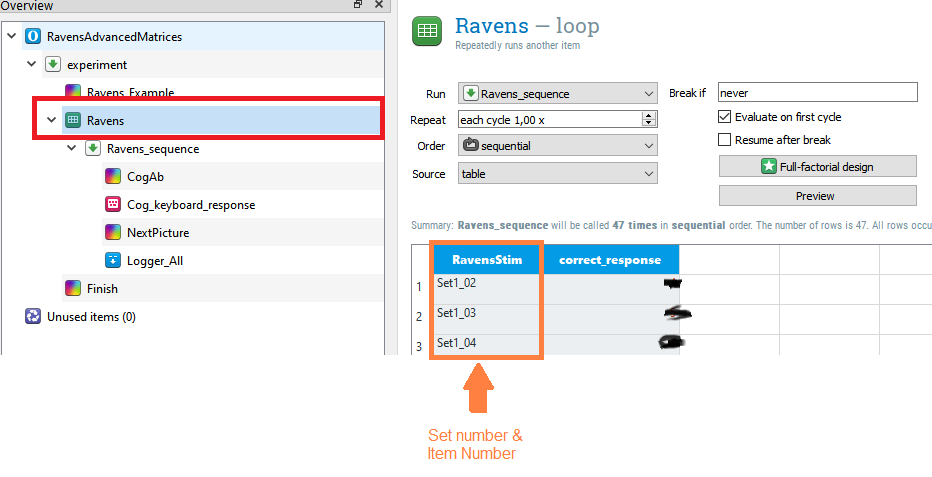
\includegraphics[width=0.99\linewidth]{images/AdvancedRPM} 

}

\caption{Remove items from the experiment by identifying them in the "Ravens" loop and deleting the corresponding row. Correct responses are blacked out.}\label{fig:Figure1-1}
\end{figure}

If you remove stimuli this way, they will no longer be shown to participants. They will, however, remain in the ``file pool'', i.e.~the folder in which Open Sesame stores the picture files. To view and/or remove these picture files, we need to access the File Pool. To do this, click on \textbf{View} -\textgreater{} \textbf{Show file pool} in Open Sesame's menu. Alternatively, press \textbf{Ctrl + P}.

As shown in Figure 2.2. below, you can view the stimuli in two different ways, either in Open Sesame or by opening the source folder. If you want to delete stimuli, highlight them in the file pool, right-click, and choose ``Delete from pool.'' In the example below, all stimuli in Set I are removed.

\begin{figure}

{\centering 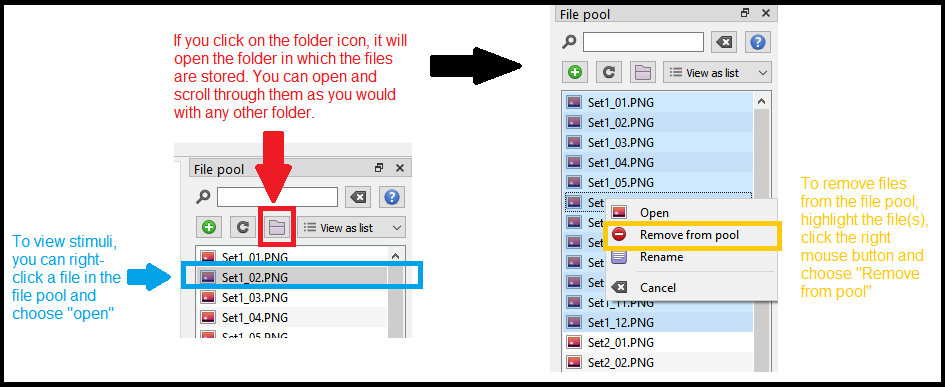
\includegraphics[width=0.99\linewidth]{images/AdvancedRPMFilePool} 

}

\caption{To view stimuli, or remove them from the Open Sesame file completely, you need to open the file pool.}\label{fig:Figure1-2}
\end{figure}

You do not have to remove pictures from the file pool as long as they have been removed from the loop. However, removing them from the file pool means the Open Sesame file of your experiment will be smaller. It is also helpful to remove any files you will not be using if you want to combine different tasks. For example, the Mill Hill Vocabulary Task and Raven's Advanced Progressive Matrices.

\hypertarget{mill-hill-vocabulary-scale}{%
\section{Mill Hill Vocabulary Scale}\label{mill-hill-vocabulary-scale}}

The Mill Hill Vocabulary Scale is a measure of linguistic ability (Raven, 2003). It contains two sets of words, Set A and Set B. The paper-based version presents participants with one of these sets as open ended questions (``What is the meaning of this word?'') and the second set as multiple choice questions. As Open Sesame does not currently support form elements for online testing, the Open Sesame files below only contain the multiple-choice version of Set A and Set B. Only one set of words should be included in an experiment.

\textbf{Formats}

The Mill Hill Vocabulary Scale Open Sesame files are suitable to be used online or offline.

Please talk to your supervisor to get the Open Sesame files.

\textbf{Things you will need to know for your Methods section}

The files for Set A and Set B both contain an example as part of the task instructions, which asks participants to identify a word similar to ``Malaria'' out of six choices: ``01 -- basement'', ``02 -- theatre'', ``03 -- ocean'', ``04 -- fever'', ``05 -- fruit'', and ``06 -- tune''. Malaria is the first word in the multiple-choice version of Set B. It is, however, also the example provided for Set A. The first multiple-choice word for Set A is currently not included in either set, to ensure an equal number of multiple-choice questions between sets.

\textbf{How to shorten the Mill Hill Vocabulary Scale?}

Watts, Baddeley, and Williams (1982) found that a shortened version of the multiple-choice part of the Mill Hill Vocabulary Scale produced reliable findings. If you want to remove items, please follow the process outlined in \emph{Shortening Raven's Advanced Progressive Matrices.}

\textbf{Ravens's Matrices \& Mill Hill References}

Matarazzo, J. D. (1990). \href{https://www.gwern.net/docs/psychology/1990-matarazzo.pdf}{Psychological assessment versus psychological testing.} \emph{American Psychologist, 45}, 999--1017.

Raven, J. (2003). Raven progressive matrices. In Handbook of nonverbal assessment (pp.~223-237). Springer, Boston, MA.

Raven, J. C. (1958). \emph{Guide to using the Mill Hill Vocabulary Scale with the Progressive Matrices Scales.} H. K. Lewis \& Co.

Watts, K., Baddeley, A., \& Williams, M. (1982). \href{https://www.sciencedirect.com/science/article/abs/pii/S0020737382800357}{Automated tailored testing using Raven's Matrices and the Mill Hill Vocabulary tests: a comparison with manual administration.} \emph{International Journal of Man-Machine Studies}, 17(3), 331-344.

\hypertarget{coloured-progressive-matrices}{%
\section{Coloured Progressive Matrices}\label{coloured-progressive-matrices}}

Raven's Coloured Progressive Matrices are similar to the Standard and Advanced Matrices. The Coloured Matrices include three sets of stimuli:

\begin{itemize}
\tightlist
\item
  \textbf{Set A:} 12 Stimuli
\item
  \textbf{Set AB:} 12 Stimuli
\item
  \textbf{Set B:} 12 Stimuli
\end{itemize}

The Coloured Matrices were originally designed for children, aged 4 to 11 years. However, if they are also suitable to be used with adults for whom the Standard Matrices may be too difficult to complete.

\textbf{Formats}

The Coloured Matrices are currently available as two different Open Sesame files. One for use on Android devices and one for use on a computer, either offline or online.

Please talk to your supervisor to get the Open Sesame files.

Using Android versions of tasks changes a few things, for example, you will to use a different Open Sesame version to make changes to it. Please check the relevant section of the Open Sesame chapter for more details.

\hypertarget{crichton-vocabulary-scale}{%
\section{Crichton Vocabulary Scale}\label{crichton-vocabulary-scale}}

The Crichton Vocabulary Scale should be used together with the Coloured Progressive Matrices. It is a measure of verbal ability and requires participants to explain words, e.g.~``What is a cap?''

\textbf{Formats}

The Crichton Vocabulary Scale Consists of open ended questions only, hence, there is no multiple-choice option available. This means, you can only use it online if you use Qualtrics. For Open Sesame, you have the option to use forms or use the Android version below.
The Android version is used by the experimenter and should not be seen by the participant. It allows you to decide whether the response was acceptable or not in real time by tapping the left or right side of a tablet screen. This may be suitable if you do not require a record of specific response.

\href{link\%20here}{Qualtrics}

For the Open Sesame file, please talk to your supervisor.

\hypertarget{working-memory-tasks}{%
\chapter{Working Memory Tasks}\label{working-memory-tasks}}

\hypertarget{digit-span-task}{%
\section{Digit Span Task}\label{digit-span-task}}

Digit Span Tasks can be used to assess working memory span. Participants are presented with a series of digits and asked to recall digits correctly. The Open Sesame Task you will find below begins with two trials that ask participants to correctly recall three digits. This number increases every two trials, until participants are asked to recall 9 digits correctly.

\textbf{Formats}

\href{GitHub/DigitSpan_Online.osexp}{Open Sesame - Offline \& Online}

\textbf{Things you will need to know for your Methods section}

Because we cannot use the form function of Open Sesame online, participants are prompted to recall digits by individual ``sketchpads'', which are similar to slides in Power Point. However, this is not the most intuitive way to respond to this task. To ensure that participants know how to respond, they complete one practice trial with three digits. They receive feedback for each individual digit and need to get all three right in order to continue to the main experiment. If they get one or more digits wrong, they are reminded of what the three digits were and invited to try again. Once they have accurately identified all three digits, they can continue to the main experiment.

\textbf{Ways to adapt the Digit Span Task}

You may want to use different numbers, letters, or even words. This can be done by opening \textbf{DigitSpan\_Loop} and changing the numbers that are entered as the digits to be shown. Figure 3.1. explains the key sections of the loop table. To see a bigger version of the image, \href{https://raw.githubusercontent.com/jmattschey/MScConversionExperiments/master/images/ChangeDigitSpan.png}{click here}

\begin{figure}

{\centering 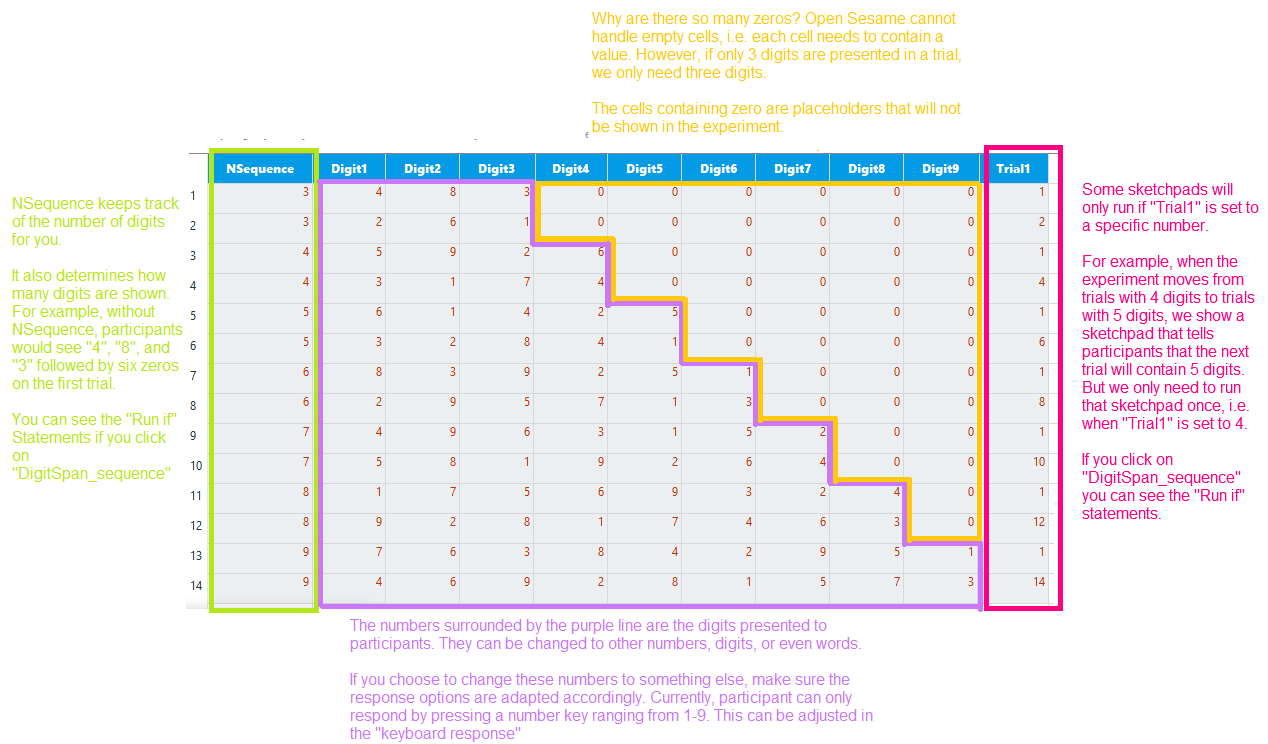
\includegraphics[width=0.99\linewidth]{images/ChangeDigitSpan} 

}

\caption{You can change the digits that are shown to participants by changig the numbers framed in purple.}\label{fig:Figure2-1}
\end{figure}

If the digits are changed to single numbers or letters, all you need to do is to adjust the allowed responses in the ``keyboard\_response'' items to allow these numbers and/or letters. If you want to use words instead, you can use the ``form'' function in Open Sesame to replace the keyboard response with. This allows participants to freely recall a word but, \textbf{importantly, the form function cannot currently be used for online experiments, as it is not supported.}

\hypertarget{attention-tasks}{%
\chapter{Attention Tasks}\label{attention-tasks}}

\hypertarget{attentional-network-task-ant}{%
\section{Attentional Network Task (ANT)}\label{attentional-network-task-ant}}

Attentional Network Tasks (ANTs) aim to assess performance in relation to the three attentional networks proposed by Posner and Petersen (1990): alerting, orienting, and executive control. The executive control network is sometimes also called ``conflict network.'' ANTs combine the cued reaction time paradigm proposed by Posner (1980) and the Eriksen Flanker Task (Eriksen, \& Eriksen, 1974). The former requires participants to identify on which side (i.e.~right or left) a target appeared, while the latter asks participants to identify a target surrounded by distractors.

The ANT included in this experiment library is based on the task version proposed by Fan, McCandliss, Sommer, Raz, and Posner (2002). The task includes five different cues. Some inform the participant that a target is about to appear and where. Others only let the the participant know that the target will appear shortly but not where. Finally, on some trials, the target will appear without a cue preceding it. Figure 4.2. shows the overview of cues participants see prior to starting the experiment.

\begin{figure}

{\centering 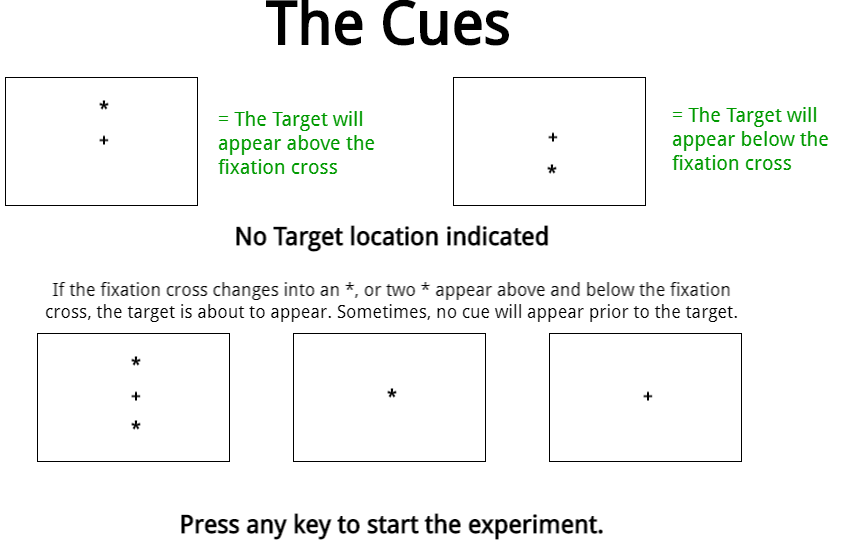
\includegraphics[width=0.8\linewidth]{images/ANT_Cues} 

}

\caption{Targets can be preceded by five different types of cues.}\label{fig:Figure3-2}
\end{figure}

The targets in this task version are arrows, which can appear either above or below the fixation cross. They are surrounded by distractor stimuli, which can either be congruent (i.e.~arrows pointing in the same direction), incongruent (i.e.~arrows pointing in the opposite direction), or neutral (in this case, a line or dash). Figure 4.3. shows the different types of target displays as they are explained to the participant.

\begin{figure}

{\centering 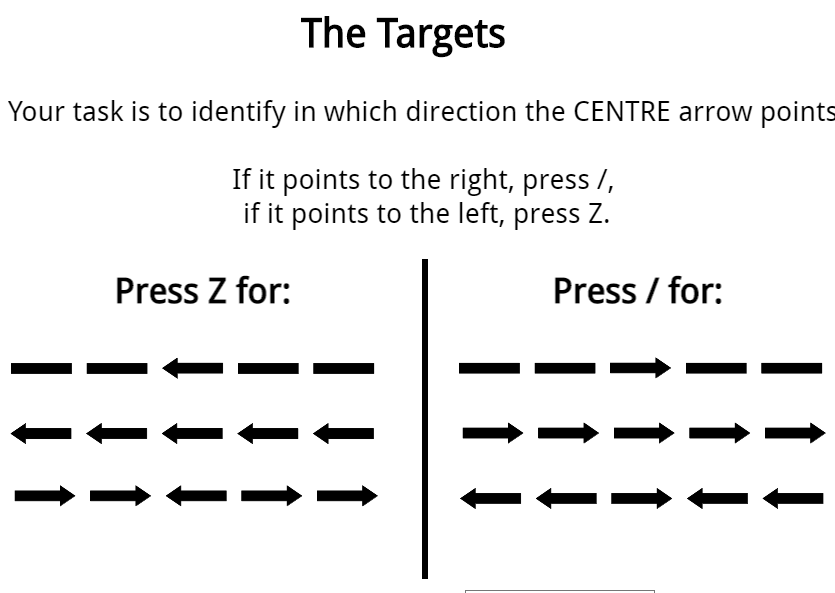
\includegraphics[width=0.8\linewidth]{images/ANT_Targets} 

}

\caption{Targets can be surrounded by congruent, incongruent, or neutral stimuli.}\label{fig:Figure3-3}
\end{figure}

\textbf{How are measures for the three attentional networks obtained?}

Performance in relation to the three networks can be assessed based on differences in reaction time and/or accuracy. This is done by comparing performance on trials with different cue types:

\begin{itemize}
\tightlist
\item
  \textbf{Alertness Network:} difference between the no-cue and the double cue condition
\item
  \textbf{Orienting Network:} difference between the centre cue and spatial cue condition
\item
  \textbf{Executive Control:} difference between trials with congruent flankers and trials with incongruent flankers
\end{itemize}

\textbf{Formats}

The task is available in two different Open Sesame formats:

\href{GitHub/ANT_OfflineWithPython.osexp}{Open Sesame Offline - Python} \textbar{} \href{GitHub/ANT_OnlineWithJS.osexp}{Open Sesame Online - JavaScript}

\textbf{Things you will need to know for your Methods section}

The ANT designed by Fan et al.~(2002) displays the first fixation cross of each trial for 400-1600ms, which is determined randomly. The display duration of the last fixation cross is determined by subtracting the duration of the first fixation cross from 3500ms. So if the first fixation cross was on screen for 500ms, the last fixation cross would be displayed for 3000ms, because 3500 - 500 = 3000. To randomly calculate these numbers, each Open Sesame file has an inline script. For the online version, it is written in Javascript, for the offline version in Python.

\textbf{ANT References}

Eriksen, B. A., \& Eriksen, C. W. (1974). \href{https://link.springer.com/content/pdf/10.3758/BF03203267.pdf}{Effects of noise letters upon the identification of a target letter in a nonsearch task.} \emph{Perception \& Psychophysics, 16}(1), 143-149.

Fan, J., McCandliss, B. D., Sommer, T., Raz, A., \& Posner, M. I. (2002). \href{http://citeseerx.ist.psu.edu/viewdoc/download?doi=10.1.1.474.442\&rep=rep1\&type=pdf}{Testing the efficiency and independence of attentional networks.} \emph{Journal of Cognitive Neuroscience, 14}(3), 340-347.

Posner, M. I., \& Petersen, S. E. (1990). \href{https://apps.dtic.mil/dtic/tr/fulltext/u2/a206157.pdf}{The attention system of the human brain.} \emph{Annual Review of Neuroscience, 13}(1), 25-42.

\hypertarget{simon-task}{%
\section{Simon Task}\label{simon-task}}

The Simon Task is based on the observation that people respond faster and with higher accuracy if the stimulus they respond to and the required response share features, for example, location (Simon, \& Wolf, 1963; Simon, \& Rudell, 1967). One version of the task requires participants to identify the colour of squares (e.g.~Gulbinaite, van Rijn, \& Cohen, 2014). Figure 4.4. shows an example of such a task. Squares are either presented on the right or left side of the screen. The response keys, M and Z, are located on the left and right side of the keyboard (if we are using a QWERTY keyboard). This means the response location (left vs.~right) and the presentation location (left vs.~right) can either match or mismatch.

\begin{figure}

{\centering 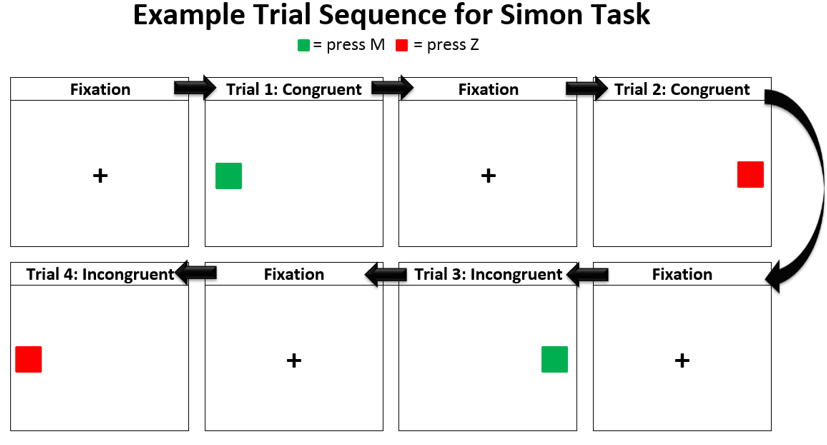
\includegraphics[width=0.8\linewidth]{images/SimonTaskExample} 

}

\caption{Example sequence of a Simon Task with coloured squares.}\label{fig:Figure3-4}
\end{figure}

If the square is red, participants should press Z, which is located on the left side of the keyboard, regardless of where the square appears. If the red square appears on the left side of the screen (i.e.~congruent trial), participants tend to be faster and commit overall fewer errors than if the red square appears on the right side of the screen (i.e.~incongruent trial).

Other variations of the task use the written words ``left'' and ``right'', or arrows.

\textbf{Formats}

The coloured square version of task is available for Open Sesame:

\href{GitHub/SimonTask.osexp}{Open Sesame - Online \& Offline}

\hypertarget{what-if-i-want-to-change-the-task-from-squares-to-arrows-or-something-else}{%
\subsection{What if I want to change the task from squares to arrows or something else?}\label{what-if-i-want-to-change-the-task-from-squares-to-arrows-or-something-else}}

Open the Simon Task and identify the following two sketchpads:

\begin{itemize}
\item
  Pract\_Target
\item
  Simon\_Target
\end{itemize}

Choose Pract\_Target and you will see something like this:

\begin{figure}

{\centering 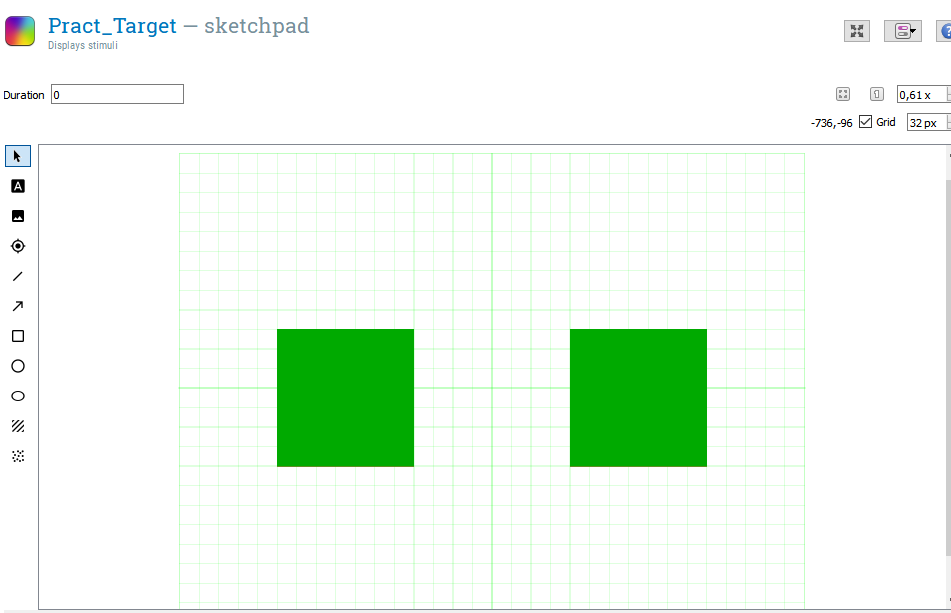
\includegraphics[width=0.99\linewidth]{images/changesimon/01Pract_Target} 

}

\caption{This is what the Target display looks like in the experiment file.}\label{fig:Figure3-5}
\end{figure}

Now we want to switch to the script view, by clicking on the functions framed in red below:

\begin{figure}

{\centering 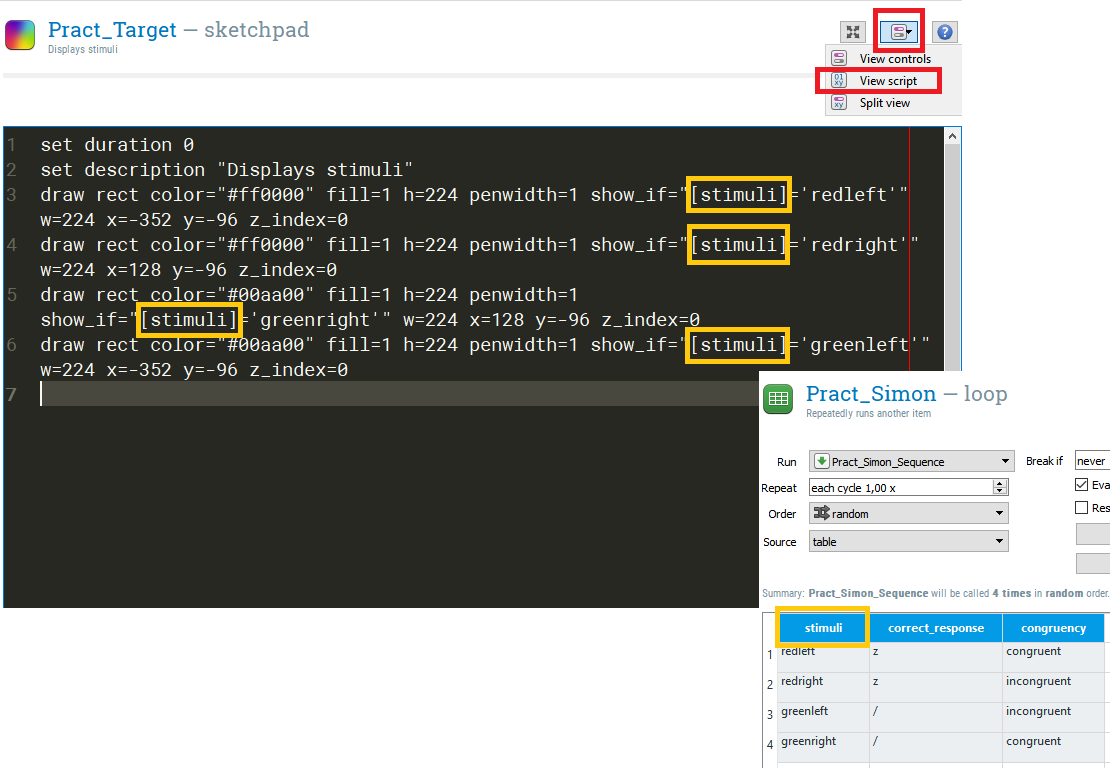
\includegraphics[width=0.99\linewidth]{images/changesimon/02Script} 

}

\caption{Every step of the experiment is based on an underlying script. This is the script that displays the targets, i.e. the coloured squares.}\label{fig:Figure3-6}
\end{figure}

You will also notice some ``show\_if'' statements framed in orange. These relate back to the Pract\_Simon loop in which we tell Open Sesame that we want four types of stimuli: a green square presented on the left or right, and a red square presented on the left or right. Now let's say we want this to change so that an arrow instead of a square is presented, e.g.~like in Stoet (2017).

Our first step is to go back to choose \textbf{``View Controls''} (between red frames in the picture above). When you are back in the control view, click on the green squares and delete them.

\url{....}

Once the squares have been removed, we can draw arrows to replace them. You can play around with the different settings to shape the arrow to your liking. Once the arrows are drawn, they can be moved around in the Control view to place them where you want them to be.

\url{....}

We want to draw four arrows: two positioned on the left, two positioned on the right. The two arrows on each side of the screen should point into opposite directions, i.e.~one points left, one points right. The arrow task version usually does not require differently coloured arrows and arrows tend to be black. You can change the colour in the the script view or in the controls view (see Figure 4.9. below).

\begin{figure}

{\centering 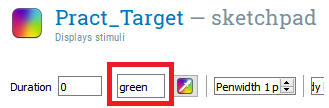
\includegraphics[width=0.6\linewidth]{images/changesimon/03SimonColour} 

}

\caption{You can change the colour of the displayed arrows in the script or control view.}\label{fig:Figure3-9}
\end{figure}

Because the arrows overlap in the control view, it can be difficult to tell them apart. However, we need to make sure that we assign the right ``show if'' argument to each arrow. One way to make this a little easier is to temporarily give each arrow a different colour.

\url{....}

Choose colours you will find easy to tell apart. The example below uses ``red'', ``green'', ``pink'' and ``blue.'' If we click on script view, we can clearly see which arrow is which.

\begin{figure}

{\centering 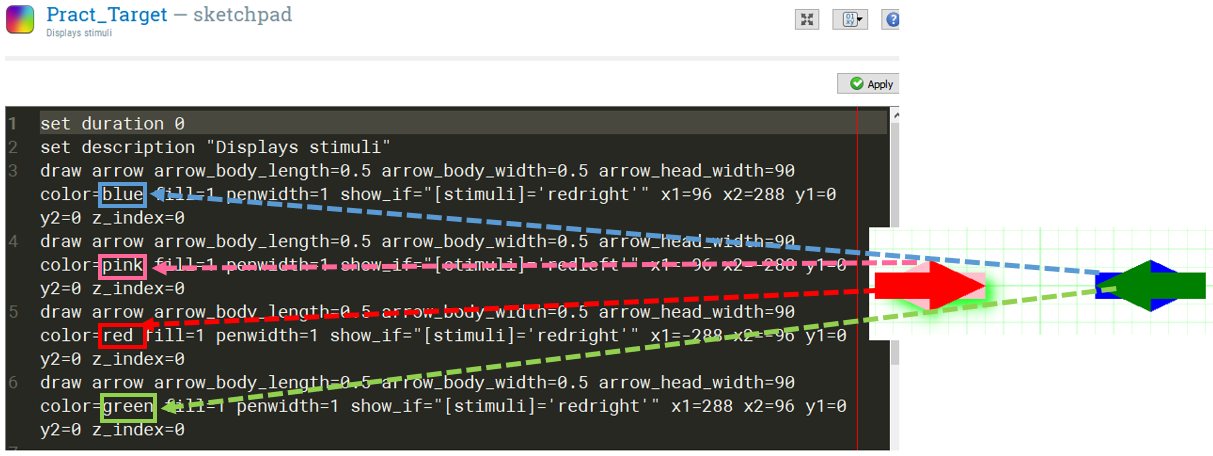
\includegraphics[width=0.99\linewidth]{images/changesimon/04colours} 

}

\caption{Close up of the four arrow colours and how they relate to the code we see in the script view.}\label{fig:Figure3-11}
\end{figure}

The next step depends on what specifically you want to ask your participants to do. For the example, we want participant to respond with Z if the arrow points left and with M if the arrow points right. To reflect this change in task, we need to change the ``stimuli'' column in the loop element:

\begin{figure}

{\centering 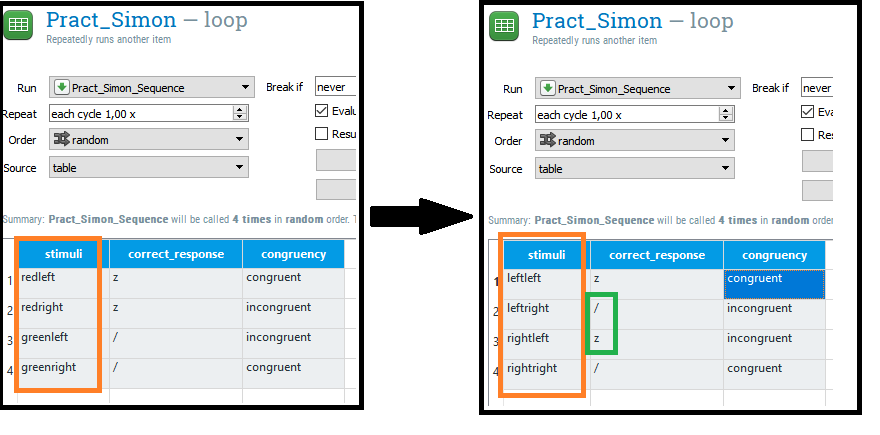
\includegraphics[width=0.99\linewidth]{images/changesimon/06Loop} 

}

\caption{We need to change the stimuli column in the loop to reflect the change in stimuli.}\label{fig:Figure3-12}
\end{figure}

The system used to name the stimuli lists the location of the arrow first, followed by its direction. Thus ``rightleft'' will draw an arrow on the right side of the screen that points towards the left. This means we also need to change the correct response in two cases (framed in green). Now that we have defined this in the loop, we can make the appropriate changes in the target sketchpad. There are two ways to do this.

\textbf{Option 1: Script view}

Go into script view and change ``show\_if'' so that the arrows are only drawn when we want them to be drawn. You will be able to tell them apart based on their colour.

\begin{figure}

{\centering 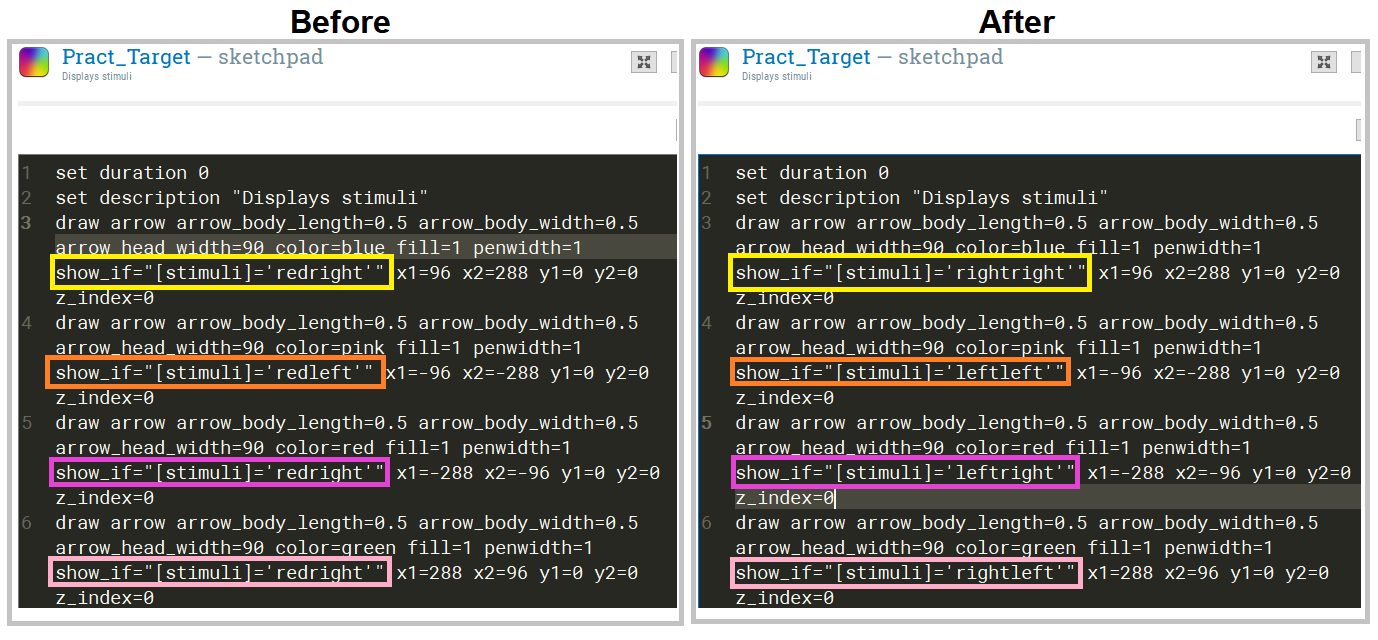
\includegraphics[width=0.99\linewidth]{images/changesimon/07script} 

}

\caption{One way to adjust the show if statement is by changing it in the script.}\label{fig:Figure3-13}
\end{figure}

After this is done, you can change to colour of all arrows to black.

\textbf{Option 2: Control view}

In the control view, click on each arrow and change the ``show if'' statement. The arrow you have selected will have a green shadow. If you choose this method, you need to be particularly careful to choose the correct arrow.

\begin{figure}

{\centering 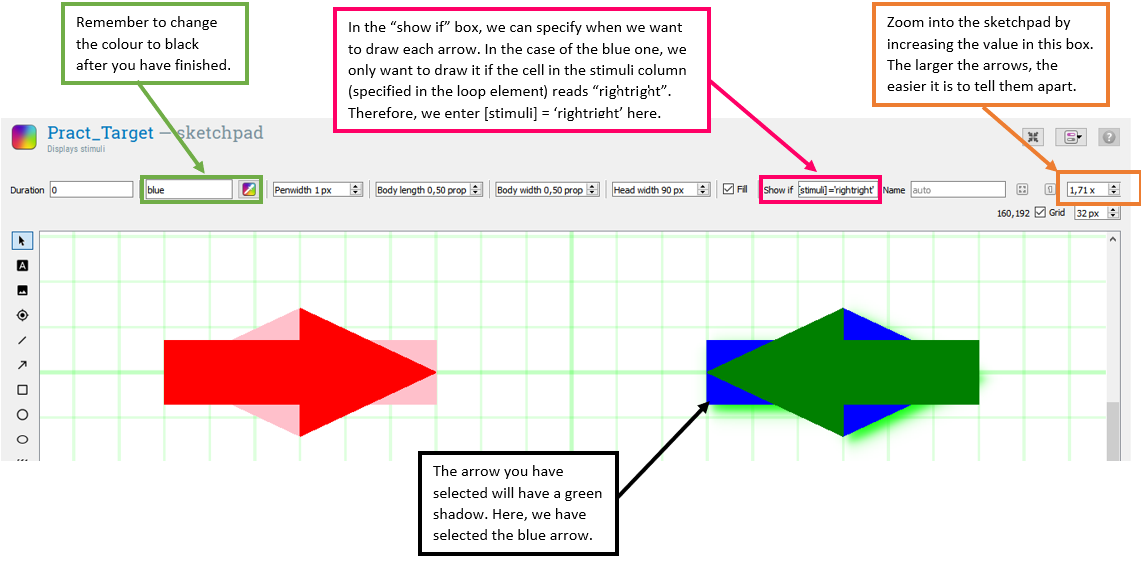
\includegraphics[width=0.99\linewidth]{images/changesimon/08option2} 

}

\caption{We can also change the show if statement in the control view.}\label{fig:Figure3-14}
\end{figure}

Once you have completed these steps, do the same for the Simon\_Block loop and the Simon\_Target sketchpad in the experimental block.

\textbf{Remember to change the instructions. Hint: You can copy-paste the script to the sketchpad in the experiment block but you still need to change the loop in the experimental block.}

\hypertarget{change-the-response-keys}{%
\subsection{Change the response keys}\label{change-the-response-keys}}

If you want to change the response keys, the first step is to change them in the loop.

\begin{figure}

{\centering 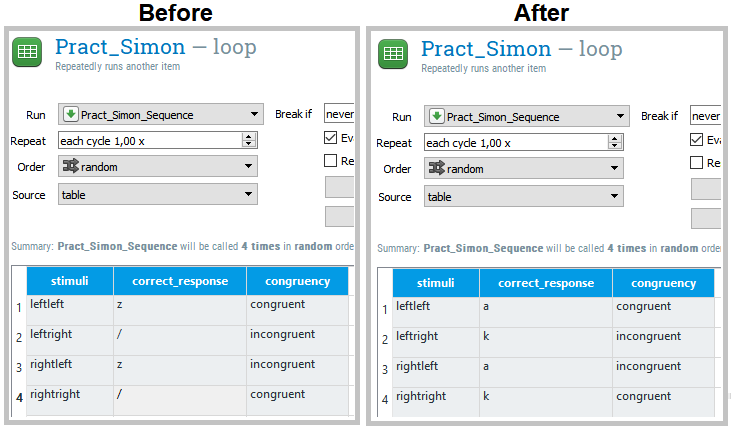
\includegraphics[width=0.99\linewidth]{images/changesimon/09response1} 

}

\caption{To change the required responses, change the correct response in the loop element.}\label{fig:Figure3-15}
\end{figure}

The second step is to change the accepted responses in the keyboard response.

\begin{figure}

{\centering 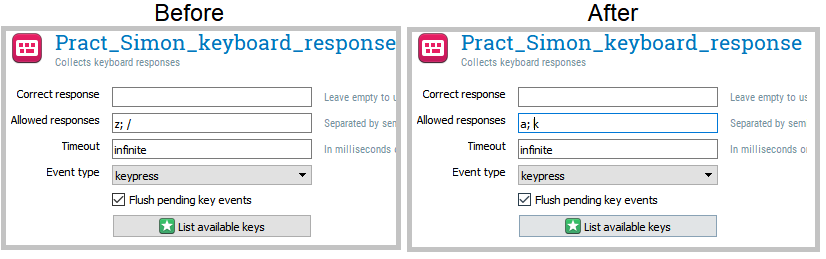
\includegraphics[width=0.99\linewidth]{images/changesimon/10response2} 

}

\caption{The second step is to change the responses we allow in the keyboard element.}\label{fig:Figure3-16}
\end{figure}

Once you have done this for the practice block, remember to do the same for the experimental block and to change the instructions accordingly.

\textbf{Simon Task References}

Gulbinaite, R., van Rijn, H., \& Cohen, M. X. (2014). \href{https://www.frontiersin.org/articles/10.3389/fnhum.2014.00761/full}{Fronto-parietal network oscillations reveal relationship between working memory capacity and cognitive control.} \emph{Frontiers in Human Neuroscience, 8}, 761.

Simon, J. R., \& Rudell, A. P. (1967). \href{https://suprimo.lib.strath.ac.uk/permalink/f/1jihtat/TN_cdi_proquest_journals_614414775}{Auditory SR compatibility: the effect of an irrelevant cue on information processing.} \emph{Journal of Applied Psychology, 51}(3), 300.

Simon, J. R., \& Wolf, J. D. (1963). {[}Choice reaction time as a function of angular stimulus-response correspondence and age.{]} (\url{https://www.tandfonline.com/doi/abs/10.1080/00140136308930679}) \emph{Ergonomics, 6}(1), 99-105.

Stoet, G. (2017). \href{https://link.springer.com/content/pdf/10.1007/s00426-016-0763-4.pdf}{Sex differences in the Simon task help to interpret sex differences in selective attention.} \emph{Psychological Research, 81}(3), 571-581.

\hypertarget{stroop-task}{%
\section{Stroop Task}\label{stroop-task}}

The Stroop Task (Stroop, 1935) is an interference control task that requires participants to identify the font colour in which colour words are written in. The word and the font colour can be either congruent, e.g.~{RED}, or incongruent, e.g.~{BLUE}. On incongruent trials, reaction time generally increases while accuracy decreases. The difference in performance between congruent and incongruent trials is also referred to as the Stroop Effect.

\textbf{Formats}

The Stroop Task is available for Open Sesame:

\href{GitHub/StroopTask.osexp}{Open Sesame - Online \& Offline}

\hypertarget{how-to-change-the-words-andor-colours}{%
\subsection{How to change the words and/or colours}\label{how-to-change-the-words-andor-colours}}

To change either the words that are displayed or the colour they are displayed in, you need to locate the Pract\_Stroop and Stroop\_Loop in the experiment file. The Figure below explains what each column defines.

\textbackslash begin\{figure\}

\{\centering 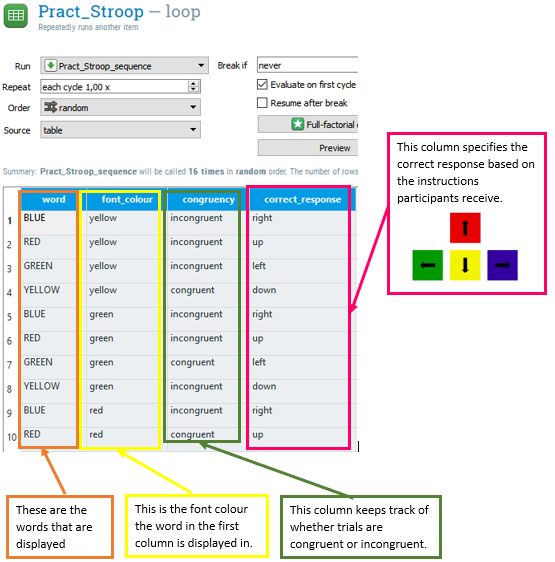
\includegraphics[width=0.99\linewidth]{images/changestroop/01loop}

\}

\textbackslash caption\{Overview of what wach column in the Pract\_Stroop loop defines.\}\label{fig:Figure3-17}
\textbackslash end\{figure\}

If you want to change the word that is displayed, for example from ``RED'' to ``PURPLE'', the words in the first column (framed in orange) needs to be changed. If you want to change the font colour, for example from {RED} to {RED}, this needs to be done in the second column, framed in yellow. Instead of colour names, you can also enter \href{https://htmlcolorcodes.com/}{Hex Colour Codes} to define the font colour. Remember that the changes you make need to reflected by the instructions you give to participants.

\textbf{Stroop References}

Stroop, J. R. (1935). \href{https://pure.mpg.de/rest/items/item_2389918/component/file_2389917/content}{Studies of interference in serial verbal reactions.} \emph{Journal of Experimental Psychology, 18}(6), 643.

\hypertarget{inhibition-of-return}{%
\section{Inhibition of Return}\label{inhibition-of-return}}

For inhibition of return (IOR) tasks, participants are expected to identify the location in which a target appeared (often right vs left side of a computer screen). The target is preceded by a cue, which appears in the same location (valid cues) or in a different location (invalid cues). If the target appears within less than 300ms after the cue, participants respond fasterand with higher accuracy on trials with valid cues (i.e.~target appears in the cued location) than on trials with invalid cues (Klein, 2000; Posner, \& Cohen, 1984). If more than 300ms lie between the cue and the target, the opposite is the case: participants respond faster if the target appears on the opposite side of where the cue appeared. In other words, if the delay between cue and target is longer than 300ms, people respond faster on invalid trials. This is also known as `validity effect.'

Thus, if the cue appears after more than around 300ms, we appear to experience suppression of our ability to orient attention to the cued location. This suppression is the ``inhibition of return'' (e.g.~to that display location). Posner and Cohen (1984) suggested that IOR facilitates the detection of novel information and may thus aid \textbf{visual search}.

\textbf{Formats}

The task is available for Open Sesame:

\href{GitHub/InhibitionofReturn.osexp}{Open Sesame - Online \& Offline}

\textbf{Things you will need to know for your Methods section}

Targets can appear 50ms, 200ms, 500ms or 800ms after the cue. You can change this by opening \textbf{``Pract\_InhibitionOfReturn\_loop''} and \textbf{``InhibitionOfReturn\_loop''} and changing the values in the \textbf{``SOA''} column.

The paradigm used in the Open Sesame task is based on Zhao and Heinke (2014) but not identical to it.

\textbf{References}

Klein, R. M. (2000). \href{https://www.researchgate.net/profile/Juan_Lupianez/publication/233995999_Inhibition_of_Return/links/0c960525d778745c66000000/Inhibition-of-Return.pdf}{Inhibition of return.} \emph{Trends in Cognitive Sciences, 4}(4), 138-147.

Posner, M. I. , \& Cohen, Y. (1984). \emph{Components of visual orienting.} In: Bouma H, Bouwhuis DG, editors. Attention and Performance X: Control of Language Processes. X. London: Lawrence Erlbaum

Zhao, Y., \& Heinke, D. (2014). \href{https://core.ac.uk/download/pdf/185482615.pdf}{What causes IOR? Attention or perception?--Manipulating cue and target luminance in either blocked or mixed condition.} \emph{Vision Research, 105}, 37-46.

\hypertarget{psycholinguistics}{%
\chapter{Psycholinguistics}\label{psycholinguistics}}

\hypertarget{lexical-decision-task}{%
\section{Lexical Decision Task}\label{lexical-decision-task}}

Lexical decision tasks require participants to identify whether a word they are presented with is a real word (e.g.~``bird'') or not (e.g.~``quapbum'').

\textbf{Formats}

The Lexical Decision Task is available for Open Sesame:

\href{GitHub/LexicalDecisionTask.osexp}{Open Sesame - Online \& Offline}

\textbf{Things you will need to know for your Methods section}

The timing of individual trials (e.g.~display time for each sketchpad) was based on Laurence, Pinto, Rosa, and Macedo (2018).

The words and non-words used in the present task were generated using the \href{https://elexicon.wustl.edu/}{English Lexicon Project}. The restricted parameters were:

\emph{For words:}

\begin{itemize}
\tightlist
\item
  Word length: 4 to 10 letters
\item
  Number of orthographic neighbours: 4 to 6
\item
  Log of Frequency of a word as reported by the HAL Study: 8 to 15
\item
  Concreteness Ratings: 4 to 5
\item
  Emotional Valence: 0 to 4
\item
  Emotional Arousal: 0 to 5
\item
  Number of Syllables: 2 to 5
\item
  Query Scope: Restricted ELP Lexicon
\end{itemize}

\emph{For non-words:}

\begin{itemize}
\tightlist
\item
  Word length: 4 to 10 letters
\item
  Orthographic neighbors that a word has: up to 15
\item
  BG\_Freq\_By\_Pos: 4750 to 5000
\item
  NWI\_Mean\_RT: 200 to 1000
\item
  NWI\_SD: up to 700
\item
  Obs: from 10
\item
  NWI\_Mean\_Accuracy: from 0.6
\end{itemize}

These restrictions produced a list of 30 words and 30 non-words. \href{extras/Lexical\%20Decision\%20Task\%20Words.xlsx}{Click here for an overview of their characteristics}

\textbf{References for Lexical Decision Task}

Laurence, P. G., Pinto, T. M., Rosa, A. T. F., \& Macedo, E. C. (2018). \href{https://prc.springeropen.com/articles/10.1186/s41155-018-0093-0}{Can a lexical decision task predict efficiency in the judgment of ambiguous sentences?} \emph{Psicologia: Reflexão e Crítica, 31}(1), 13.

\hypertarget{assessig-degree-of-bilingualism}{%
\section{Assessig Degree of Bilingualism}\label{assessig-degree-of-bilingualism}}

The Language and Social Background Questionnaire (LSBQ) aims to provide an indication of how bilingual or monolingual a person is. It considers how frequently people use different languages, how proficient they are, and in what contexts they use different languages.

\textbf{Formats}

The LSBQ is analysed through an Excel spreadsheet, which can be downloaded \href{https://figshare.com/articles/The_Language_and_Social_Background_Questionnaire_Assessing_Degree_of_Bilingualism_in_a_Diverse_Population_Supplementary_Materials/3972486}{here}. Along with the Excel spreadsheet, a PDF in English is available.

\textbf{References for LSBQ}

Anderson, J. A., Mak, L., Chahi, A. K., \& Bialystok, E. (2018). \href{https://link.springer.com/article/10.3758/s13428-017-0867-9}{The language and social background questionnaire: Assessing degree of bilingualism in a diverse population.} \emph{Behavior Research Methods, 50}(1), 250-263.

\hypertarget{spatial-awareness}{%
\chapter{Spatial Awareness}\label{spatial-awareness}}

\hypertarget{mental-rotation}{%
\section{Mental Rotation}\label{mental-rotation}}

During mental rotation tasks, participants are generally presented with two objects and asked to identify whether these objects are the same or different. The objects can be two-dimensional and three-dimensional, and one image is rotated by a few degrees (e.g.~50°, 100°,\ldots) compared to the other. Below is an example image from the data set used in the Open Sesame task you can download below.

\begin{figure}

{\centering 
\includegraphics[width=0.75\linewidth]{images/RotationExample} 

}

\caption{Example of the stimuli used in the Open Sesame task that can be downloaded below. The stimuli were created by Ganis and Kievit (2015) and shared as an open dataset.}\label{fig:Figure5-1}
\end{figure}

\textbf{Formats}

The mental rotation task, with the stimuli created by Ganis and Kievit (2015), is available as a short and long Open Sesame file. The short version contains 96 stimuli pairs, the long version contain all 384 stimuli created by Ganis and Kievit.

Both are suitable to be used online, however, the long task version can be expected to take around 30 minutes to complete, which is quite long for an online
study.

\href{GitHub/SpatialRotationShort.osexp}{Open Sesame - Short Version} \textbar{} \href{GitHub/SpatialRotationLong.osexp}{Open Sesame - Long Version}

\textbf{Things you will need to know for your Methods section}

Remember to cite Ganis and Kievit (2015) as the source of the stimuli. Check their article for details of how the stimuli were created. The set they created includes 48 objects, each compared to itself and a different object rotated by 0°, 50°, 100°, and 150°. This means that for each angle and object, there is a pair of objects that are the same and a pair that shows two different objects. Below shows Object 1 and its corresponding pairs of stimuli as an example.

\begin{figure}

{\centering 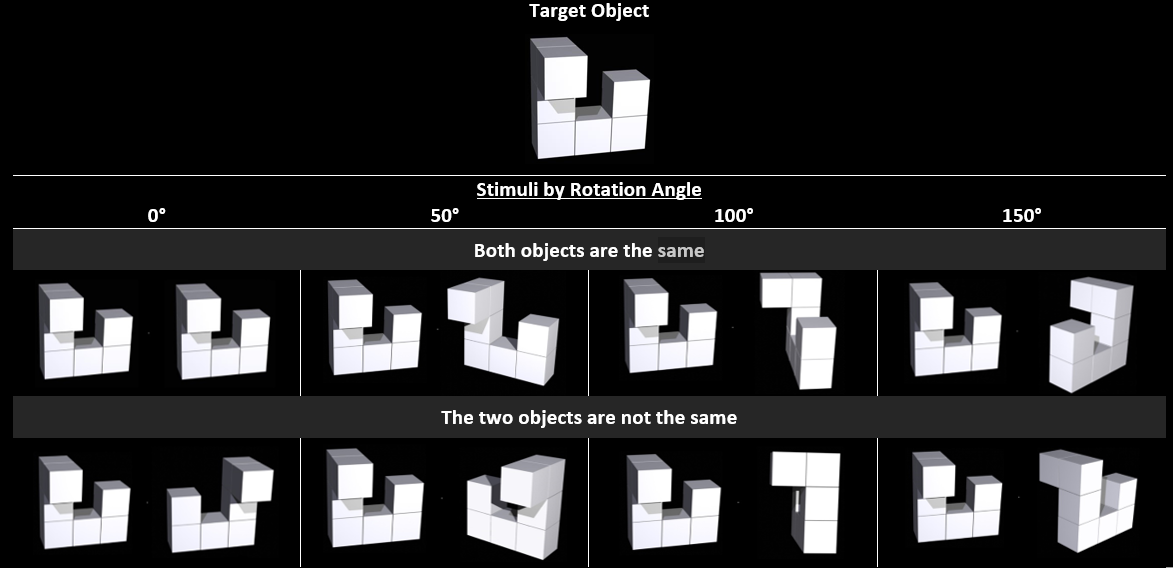
\includegraphics[width=0.99\linewidth]{images/RotationOverview} 

}

\caption{Object 1 in the stimuli set created by Ganis and Kievit (2015). Each Object features in 8 picture pairs. Four of these pairs show the same object twice but at different rotation angles. The other four pictures show the object next to a different object, also at different degrees of rotation.}\label{fig:Figure5-2}
\end{figure}

The long task version includes all 384 pairs of objects, half showing matching pairs, half showing mismatching pairs. The four angles (0°, 50°, 100°, and 150°) are evenly distributed, which means there are 96 pairs of objects for each angle. The shorter version only includes 96 pairs total, half of which are also matching and half of which are mismatching. It includes 24 object pairs for each angle.

The shorter set of pictures was created by putting the list of stimuli file names into an alphabetical order. As shown in the picture below, each image file in Ganis and Kievit's set of stimuli is labeled with the object number first, followed by the rotation angle. In half the cases this is then followed by an ``R'' at the end. The pairs without an R at the end of the file name show matching pairs of objects, i.e.~both objects are the same. The file names of images that show two different objects end with an R. For example, ``6\_150'' refers to the image that shows object 6 and object 6 rotated by 150°. ``6\_150\_R'' refers to the image that shows objects 6 next to a different object that is rotated by 150°.

\begin{figure}

{\centering 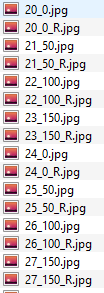
\includegraphics[width=0.2\linewidth]{images/RotationNumberList} 

}

\caption{Example of the object pairs included in the short task version, as shown in the file pool in Open Sesame.}\label{fig:Figure5-3}
\end{figure}

The short task version only contains two pictures of each object, both with the same rotation angle, however, one shows a matching pair of objects and one shows a mismatching pair. For example, for object 21, only the two pictures with a 50° rotation were kept. Sorting file names alphabetically, rotation increased with each object.

For example, for object 20, the two pictures in which the second object was rotated by 0° were kept. For object 21, the two pictures with objects rotated by 50° were included, for object 22 the two pictures with objects rotated by 100° were chosen, and for object 23, the two pictures with object rotated by 150° stayed in the set of stimuli. This continued, with the two pictures with objects rotated by 0° being include for object 24, and so on. The whole list of included objects can be seen in the file pool in Open Sesame. To access the file pool, open the experiment in Open Sesame and click on \textbf{View} -\textgreater{} \textbf{Show file pool} in Open Sesame's menu. Alternatively, press \textbf{Ctrl + P}.

\textbf{References}

Ganis, G., \& Kievit, R. (2015). \href{https://openpsychologydata.metajnl.com/articles/10.5334/jopd.ai/}{A new set of three-dimensional shapes for investigating mental rotation processes: validation data and stimulus set.} \emph{Journal of Open Psychology Data, 3}, e3

\hypertarget{social-psychology-tasks}{%
\chapter{Social Psychology Tasks}\label{social-psychology-tasks}}

\hypertarget{implicit-association-task-iat}{%
\section{Implicit Association Task (IAT)}\label{implicit-association-task-iat}}

Implicit Association Tasks (IATs) require participants to categorise words as fast as possible into one of two categories (e.g.~pleasant vs.~unpleasant). In general, faster responses suggest stronger implicit associations. After some practice blocks with only two options, participants are expected to be familiar with the target words and asked to sort them while four different target categories are present. These categories are paired, e.g.~``female - pleasant'', ``male - unpleasant.'' If the paired categories match the associations held by the participant, reaction times tend to be faster. For example, if participants have positive associations with the word and/or category female, they would be expected to respond faster if ``female'' and ``pleasant are displayed together than if''female" and "unpleasant are displayed together.

\textbf{Formats}

A task version looking at gender and maths/language studies association can be downloaded for Open Sesame. The task that can be downloaded combines the paradigms used by Smeding et al.~(2016) and Nosek, Banaji, and Greenwald (2016).

\href{GitHub/ImplicitAssociationTask.osexp}{Open Sesame Online and Offline}

\textbf{Things you will need to know for your Methods section}

The task uses the male/female and math/language stimuli used by Smeding et al.~(2016).

The block design is as follows:

\begin{figure}

{\centering 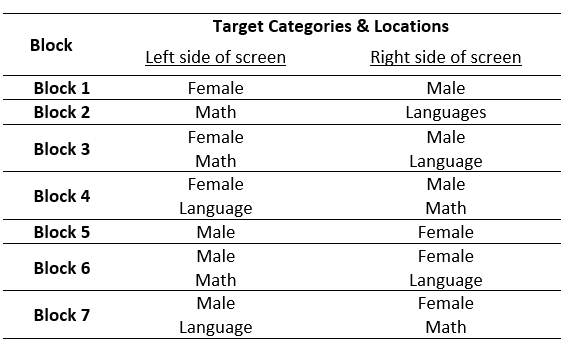
\includegraphics[width=0.75\linewidth]{images/IAT_Design} 

}

\caption{Overview of IAT blocks.}\label{fig:Figure6-1}
\end{figure}

\textbf{References}

Smeding, A., Quinton, J. C., Lauer, K., Barca, L., \& Pezzulo, G. (2016). \href{https://www.researchgate.net/profile/Jean-Charles_Quinton/publication/308341625_Tracking_and_Simulating_Dynamics_of_Implicit_Stereotypes_A_Situated_Social_Cognition_Perspective/links/581b4c3508aea429b28fc0d0/Tracking-and-Simulating-Dynamics-of-Implicit-Stereotypes-A-Situated-Social-Cognition-Perspective.pdf}{Tracking and simulating dynamics of implicit stereotypes: A situated social cognition perspective.} \emph{Journal of Personality and Social Psychology, 111}(6), 817.

Nosek, B.A., Banaji, M.R., \& Greenwald, A.G. (2002). \href{https://psyarxiv.com/y2g6s}{Math = Male, Me = Female, therefore Math ¹Me.} \emph{Journal of Personality and Social Psychology, 83}, 44-59

\hypertarget{questionnaires-copyright}{%
\chapter{Questionnaires \& Copyright}\label{questionnaires-copyright}}

The questionnaires included in this Experiment Library are subject to different licence agreements. In general, though, they can be used if the original source is acknowledged as part of your work. Thus, if you want to use any of these questionnaires, \textbf{it is vital that you quote the article that relates to it.}

\hypertarget{personality-questionnaires}{%
\chapter{Personality Questionnaires}\label{personality-questionnaires}}

\hypertarget{big-5}{%
\section{Big 5}\label{big-5}}

The `Big 5' is a term that relates to five personality dimensions: Extraversion,
Conscientiousness, Openness, Agreeableness and Neuroticism. Neuroticism is also sometimes called `emotional stability.' Several different questionnaires have been developed to study the Big 5, including the TIPI described below.

\hypertarget{ten-item-personality-inventory-tipi}{%
\subsection{Ten-Item Personality Inventory (TIPI)}\label{ten-item-personality-inventory-tipi}}

The TIPI is a short questionnaire that can be used to study the Big 5 personality dimensions. It was developed by Gosling, Rentfrow, and Swann (2003).

\textbf{How to use the TIPI}

The TIPI includes, as the name suggests, 10 items. Each item asks participants to rate their response on a scale from 1 (Disagree strongly) to 7 (Agree Strongly). The TIPI includes two items related to each personality dimension, including one that is scored in reverse (marked by the R behind the item number below).

\begin{itemize}
\tightlist
\item
  \emph{Extraversion}: 1, 6R
\item
  \emph{Agreeableness:} 2R, 7
\item
  \emph{Conscientiousness:} 3, 8R
\item
  \emph{Neuroticism:} 4R, 9
\end{itemize}

The positively scored item is simply scored by recording the number the participant indicated. For example, if a participant strongly disagreed with a statement, we would record ``1'' as the value for that question. If the item is scored in reverse, ``strongly disagree'' would be scored with a 7 instead.

\emph{Converting the reverse items:}

1=7; 2=6; 3=5;, 4=4; 5=3; 6=2; 7=1

\textbf{Formats}

The TIPI can be downloaded in the following formats:

\href{questionnaires/10-ItemPersonalityInventory_TIPI.docx}{Word} \textbar{} \href{questionnaires/10-ItemPersonalityInventory_TIPI.qsf}{Qualtrics}

The Qualtrics file will provide scores for each dimension and score reversed items in reverse.

\textbf{Source:}

Gosling, S. D., Rentfrow, P. J., \& Swann Jr., W. B. (2003). \href{http://citeseerx.ist.psu.edu/viewdoc/download?doi=10.1.1.113.6704\&rep=rep1\&type=pdf}{A very brief measure of the Big-Five personality domains.} \emph{Journal of Research in Personality, 37,} 504-528.

\hypertarget{emotions}{%
\section{Emotions}\label{emotions}}

\hypertarget{humor-styles-questionnaire-hsq}{%
\subsection{Humor Styles Questionnaire (HSQ)}\label{humor-styles-questionnaire-hsq}}

Humour is considered an emotional measure. It is possible to distingush between different kinds of humour, for example, sarcasm or banter. The Humor Styles Questionnaire (HSQ) was developed by Marting et al.~(2003) and distinguishes four styles of humour:

\begin{enumerate}
\def\labelenumi{\arabic{enumi}.}
\tightlist
\item
  \emph{Self-enhancing Humour:} Humour used to enhance the self, without any detriment to the self or others
\item
  \emph{Affiliative Humour:} Humour used to enhance the relationship with other people
\item
  \emph{Aggressive Humour:} Use of humour to the detriement/at the expense of others
\item
  \emph{Self-defeating Humour:} Use of humour to the detriement/at the expense of the self
\end{enumerate}

\textbf{How to use the HSQ}

The HSQ contains 32 items and each type of humour is measured by 8 of these. Each item is scored from 1 (Totally Disagree) to 7 (Totally Agree). Some of these items are scored in reverse (marked by an R in the list below). For example, if a participants chooses ``3'' (Slightly Disagree") for a reverse item, we would use 5 as the score.

\emph{Converting the reverse items:}

1=7; 2=6; 3=5;, 4=4; 5=3; 6=2; 7=1

Items for each subscale:

\begin{itemize}
\tightlist
\item
  \emph{Affiliative Humour:} 1R, 5, 9R, 13, 17R, 21, 25R, 29R
\item
  \emph{Self-Enhancing Humour:} 2, 6, 10, 14, 18, 22R, 26, 30
\item
  \emph{Aggressive Humour:} 3, 7R, 11, 15R, 19, 23R, 27, 31R
\item
  \emph{Self-Defeating Humour:} 4, 8, 12, 16R, 20, 24, 28, 32
\end{itemize}

\textbf{Formats}

The HSQ can be downloaded as paperbased version or for Qualtrics.

\href{questionnaires/HumorStylesQuestionnaire.docx}{Word} \textbar{} \href{questionnaires/HumorStylesQuestionnaire.qsf}{Qualtrics}

The Qualtrics file is set up to calculate the score for each sub-category of humour. Reversed items are scored in reverse if you use the Qualtrics file.

\textbf{Source:}

Martin, R.A., Puhlik-Doris, P., Larsen, G., Gray, J., \& Weir, K. (2003). \href{https://d1wqtxts1xzle7.cloudfront.net/56892479/HSQ_article.pdf?1530281324=\&response-content-disposition=inline\%3B+filename\%3DIndividual_differences_in_uses_of_humor.pdf\&Expires=1598969255\&Signature=c2oQ1bWDYeWlwZslWOqrGvNdgjeYek-qW6UbPTZVWozQfdWJ8HAKPZHZRSACz1mNY6TYSVsbQgCYsC~1vG7IWPHEnUyQtT2cWsljBOMDj-m6KECtv9OSsQqBWQqTbOQbaGbyRGaCJbbdYEPr4uNZM8zVWZWB0cQU105xtYzzrqyrEQvnR-8x7Y2-7pCwPBMptT8CLRgiv4~WEz1auOoHClqgZ0pAg6Qe8oTVIYFaX40f0gT2At1JKH-xmb1-IHX7wWz9zux-3WMYZ0~jNi4kruIbEHnSS6HrAmF-sin3lWpItwnvWRJ2XbJEFvaU3HqsWTdmsM2WpnIwBQ8I5mCKpw__\&Key-Pair-Id=APKAJLOHF5GGSLRBV4ZA}{Individual differences in uses of humor and their relation to psychological well-being: Development of the Humor Styles Questionnaire.} \emph{Journal of Research in Personality, 37}, 48-75.

\hypertarget{oxford-happiness-questionnaire-ohq}{%
\subsection{Oxford Happiness Questionnaire (OHQ)}\label{oxford-happiness-questionnaire-ohq}}

As the name suggests, the Oxford Happiness Questionnaire (OHQ) aims to measure happiness. It was developed by Hills and Argyle (2002), based on the Oxford Happiness Inventory. The QHQ contains 29 items, however, Hills and Argyle (2002) found that a subset of eight items was suitable to classify around 90\% of responses accurately.

\textbf{How to use the QHQ}

The QHQ contains 29 items, each of which participants score between 1 (strongly disagree) to 6 (strongly agree). Twelve of these items are scored in reverse.

\emph{The following items are scored in reverse:}

1, 5, 6, 10, 13, 14, 19, 23, 24, 27, 28, 29

\emph{Converting the reverse items:}

1=6; 2=5; 3=4;, 4=3; 5=2; 6=1

The items included in the \textbf{8-item version} proposed by Hills and Argyle (2002) are: 1, 3, 12, 13, 16, 18, 21, and 29

\textbf{Formats}

The full QHQ is available to download as Word document, the 8-item version can be downloaded as Word document or Qualtrics file.

\href{questionnaires/OxfordHappinessQuestionnaire.docx}{Word - full QHQ} \textbar{} \href{questionnaires/OxfordHappinessQuestionnaire_8ItemVersion.docx}{Word - 8-item QHQ} \textbar{} \href{questionnaires/OxfordHappinessQuestionnaire_8ItemVersion.qsf}{Qualtrics - 8-item}

\textbf{Source}

Hills, P., \& Argyle, M. (2002). \href{https://pdfs.semanticscholar.org/cadd/7a4eea79e031ec0cf8b8054f668057f33dda.pdf}{The Oxford Happiness Questionnaire: a compact scale for the measurement of psychological well-being.} \emph{Personality and Individual Differences, 33}(7), 1073-1082.

\hypertarget{satisfaction-with-life-scale-swls}{%
\subsection{Satisfaction with life scale (SWLS)}\label{satisfaction-with-life-scale-swls}}

The Satisfaction with life scale (SWLS) was developed by Diener, Emmons, Larsen, and Griffin (1985). It aims to measure how satisfied someone is with their life in general.

As mentioned in Chapter 8, you should always cite the source of a questionnaire but it is worth noting the official re-use statement from the \href{http://labs.psychology.illinois.edu/~ediener/SWLS.html}{official SWLS website}:

\emph{`The scale is copyrighted but you are free to use it without permission or charge by all professionals (researchers and practitioners) as long as you give credit to the authors of the scale: Ed Diener, Robert A. Emmons, Randy J. Larsen and Sharon Griffin as noted in the 1985 article in the Journal of Personality Assessment.'}

\textbf{How to use the SWLS}

Each of the five items included in the SWLS is rated on a scale from 1 (Strongly disagree) to 7 (Strongly Agree). There are \textbf{no} reverse items included in the scale, thus, the possible scores range from 5 to 35.

Diener et al.~(1985) propose the following classifications:

\begin{itemize}
\tightlist
\item
  \emph{5 to 9:} Extremely Dissatisfied
\item
  \emph{10 to 14:} Dissatisfied
\item
  \emph{15 to 19:} Slightly below average life satisfaction
\item
  \emph{20 to 24:} Average score/Average life satisfaction
\item
  \emph{25 to 29:} High score/High life satisfaction
\item
  \emph{30 to 35:} Very high score/ Very high life satisfaction
\end{itemize}

A detailed guide on how to interpret the findings can be found on the \href{http://labs.psychology.illinois.edu/~ediener/SWLS.html}{official SWLS website}.

Kobau et al.~(2010) developed a version of the SWLS with a 5-point response scale, which may be of interest to some.

\textbf{Formats}

The SWLS can be downloaded from the \href{http://labs.psychology.illinois.edu/~ediener/SWLS.html}{official website}, in a wide range of different lanuages.

\href{/questionnaires/Satisfaction_of_Life_Scale}{Qualtrics}

\textbf{Source \& References}

Diener, E., Emmons, R. A., Larsen, R. J., \& Griffin, S. (1985). \href{https://emmons.faculty.ucdavis.edu/wp-content/uploads/sites/90/2015/08/1985_5-SWLS.pdf}{The Satisfaction with Life Scale}. \emph{Journal of Personality Assessment, 49}, 71-75.

Kobau, R., Sniezek, J., Zack, M. M., Lucas, R. E., \& Burns, A. (2010). \href{https://iaap-journals.onlinelibrary.wiley.com/doi/abs/10.1111/j.1758-0854.2010.01035.x.*Applied\%20Psychology:\%20Health\%20and\%20Well-being}{Well‐being assessment: An evaluation of well‐being scales for public health and population estimates of well‐being among US adults}, 2*(3), 272-297.

\hypertarget{relationships}{%
\section{Relationships}\label{relationships}}

\hypertarget{romantic-jealousy-multi-dimensional-jealousy-scale}{%
\subsection{Romantic Jealousy (Multi-dimensional Jealousy Scale)}\label{romantic-jealousy-multi-dimensional-jealousy-scale}}

The Multi-Dimensional Jealousy Scale (MJS) was developed by Pfeiffer and Wong (1989) and aims to assess jealousy along three dimensions:

\begin{enumerate}
\def\labelenumi{\arabic{enumi}.}
\tightlist
\item
  \emph{Cognitive Jealousy:} How frequently someone experiences thoughts or worries related to jealousy
\item
  \emph{Emotional Jealousy:} Feelings people experience in relation to jealousy
\item
  \emph{Behavioral Jealousy:} How often someone engages in jealous behaviour, e.g.~checking a partner's private belongings.
\end{enumerate}

More recently, Elphinston, Feeney and Noller (2011) developed a shorter version of the MJS, which contains only 17 items instead of the 24 items included in the full MJS.

\textbf{How to use the MJS}

The MJS includes 8 items for each jelousy dimension, i.e.~a total of 24 items. Participants are asked to rate their response on a scale from 1 to 7.

For the items related to Cognitive Jealousy and Behavioural Jealousy, the response labels range from 1 (never) to 7 (all the time). For Emotional Jealousy, they range from 1 (very pleased) to 7 (very upset).

\textbf{Formats}

The MJS is available in the following formats:

\href{questionnaires/Multi-dimensionalJealousyScale.docx}{Word} \textbar{} \href{questionnaires/Multi-dimensionalJealousyScale.qsf}{Qualtrics}

It is worth mentioning that some items use the phrases such as \emph{`attracted to the opposite sex'} and may need to be adapted for use with non-heterosexual participants.

Some items of the MJS, e.g.~\emph{`I suspect that X may be attracted to someone else'}, suggest it may only be reliable for people in monogamous relationships. If this questionnaire is used, it would therefore be advisable to include a question to confirm the type of relationship participants are in.

\textbf{Source:}

Elphinston, R. A., Feeney, J. A., \& Noller, P. (2011). \href{https://aps.onlinelibrary.wiley.com/doi/abs/10.1111/j.1742-9536.2011.00026.x}{Measuring romantic jealousy: Validation of the multidimensional jealousy scale in Australian samples.} \emph{Australian Journal of Psychology, 63}(4), 243-251.

Pfeiffer, S. M., \& Wong, P. T. P. (1989). \href{http://www.drpaulwong.com/wp-content/uploads/2018/03/Multidimensional-Jealousy-Scale-Pfeiffer-Wong-1989-Paper.pdf}{Multidimensional jealousy.} \emph{Journal of Social and Personal Relationships, 6}, 181-196.

\hypertarget{state-adult-attachment-measure-saam}{%
\subsection{State Adult Attachment Measure (SAAM)}\label{state-adult-attachment-measure-saam}}

Attachment styles can generally be described as Secure, Anxious, or Avoidant, with some researchers also differentiating between dismissive avoidant and fearful avoidant attachment styles. The State Adult Attachment Measure (SAAM) can be used to study attachment styles of adults.

\textbf{How to use the SAAM}

The SAAM contains 21 questions, which items relating to Secure, Anxious, and Avoidant behaviour. The Word document version of the questionnaire available from the \href{http://gillab.ku.edu/resources}{authors lab website} clearly states which item relates to which sub-scale.

The SAAM includes 7 items for each attachment style, which are rated on a scale from 1 (disagree strongly) to 7 (agree strongly). There are \textbf{no} reverse items included.

\textbf{Formats}

A Word document version of the SAAM can be downloaded from the \href{http://gillab.ku.edu/resources}{Gillath Lab website}

\href{questionnaires/State_Adult_Attachment_Measure_SAAM.qsf}{Qualtrics}

\textbf{Sources:}

Gillath, O., Hart, J., Noftle, E. E., \& Stockdale, G. D. (2009). \href{https://www.researchgate.net/profile/Omri_Gillath/publication/223185973_Development_and_validation_of_a_State_Adult_Attachment_Measure_SAAM/links/5a10d5c2458515cc5aa8073c/Development-and-validation-of-a-State-Adult-Attachment-Measure-SAAM.pdf}{Development and validation of a state adult attachment measure (SAAM).} \emph{Journal of Research in Personality, 43}, 362-373.

\hypertarget{political-tendency}{%
\section{Political Tendency}\label{political-tendency}}

\hypertarget{social-and-economic-conservatism-scale-secs}{%
\subsection{Social and Economic Conservatism Scale (SECS)}\label{social-and-economic-conservatism-scale-secs}}

The Social and Economic Conservatism Scale (SECS) developed by Everett (2013) aims to estimate political conservatism. What constitutes political conservatism varies often by geographical location. The SECS was developed with the United States in mind but has also previously been used for research in the United Kingdom (e.g.~Banton, West, \& Kinney, 2020).

\textbf{How to use the SECS}

The SECS requires participants how positive or negative they feel about a topic, e.g.~the military, on a sliding scale from 0 to 100. On this scale, 50 would be considered neutral, 0 negative, and 100 positive. The SECS contains 12 items which are scored in this way.

\textbf{Formats}

The SECS is available in the following formats:

\href{/questionnaires/SocialandEconomicConservatismScale.docx}{Word} \textbar{} \href{/questionnaires/SocialandEconomicConservatismScale.qsf}{Qualtrics}

\textbf{Source \& References}

Banton, O., West, K., \& Kinney, E. (2020). \href{https://onlinelibrary.wiley.com/doi/pdf/10.1111/bjso.12337}{The surprising politics of anti‐immigrant prejudice: How political conservatism moderates the effect of immigrant race and religion on infrahumanization judgements.} \emph{British Journal of Social Psychology, 59}(1), 157-170.

Everett, J. A. (2013). \href{https://journals.plos.org/plosone/article/file?id=10.1371/journal.pone.0082131\&type=printable}{The 12 item social and economic conservatism scale (SECS).} \emph{PloS ONE, 8}(12), e82131.

\hypertarget{personality-disorders}{%
\section{Personality Disorders}\label{personality-disorders}}

\hypertarget{levenson-self-report-psychopathy-scale-lsrp}{%
\subsection{Levenson Self-Report Psychopathy Scale (LSRP)}\label{levenson-self-report-psychopathy-scale-lsrp}}

The Levenson Self-Report Psychopathy Scale (LSRP) was developed by Levenson, Kiehl, and Fitzpatrick (1995). It measures two types of Psychopathy:

\begin{enumerate}
\def\labelenumi{\arabic{enumi}.}
\tightlist
\item
  \emph{Primary Psychopathy}: Callous and unemotional attitudes and/or behaviour, usually low level of anxiety
\item
  \emph{Secondary Psychopathy}: Being implusive and engaging in self-destructive behaviour, often accompanied by high levels of anxiety
\end{enumerate}

\textbf{How to use the LSRP}

The LSRP contains a total of 26 items, including 16 related to Primary Psychopathy and 10 related to Secondary Psychopathy. Each item is rated on a 4-point response scale:

\begin{itemize}
\tightlist
\item
  1 = disagree strongly
\item
  2 = disagree somewhat
\item
  3 = agree somewhat
\item
  4 = agree strongly
\end{itemize}

The following items included in the Primary Psychopathy section are scored in reverse: 10, 12, 14, 15, 16.

In the Secondary Psychopathy section, the following items are scored in reverse: 3, 7

\textbf{Formats}

The LSRP is available in the following formats:

\href{/questionnaires/LevensonSelf-ReportPsychopathyScale_LSRP.docx}{Word} \textbar{} \href{/questionnaires/LevensonSelf-ReportPsychopathyScale_LSRP.qsf}{Qualtrics}

\textbf{Source:}

Levenson, M. R., Kiehl, K. A., \& Fitzpatrick, C. M. (1995). \href{https://www.researchgate.net/profile/Michael_Levenson2/publication/15338539_Assessing_Psychopathic_Attributes_in_a_Noninstitutionalized_Population/links/54b6d8360cf2bd04be334b31.pdf}{Assessing psychopathic attributes in a noninstitutionalized population.} \emph{Journal of Personality and Social Psychology, 68}(1), 151.

\hypertarget{brief-histrionic-personality-scale-bhps}{%
\subsection{Brief Histrionic Personality Scale (BHPS)}\label{brief-histrionic-personality-scale-bhps}}

Histrionic Personality disorder is associated with attention-seeking and egocentric behaviour. The Brief Histrionic Personality Scale (BHPS) was developed by Ferguson and Negy (2014) and aims to give an indication of whether a person may be affected by it.

\textbf{How to use the BHPS}

The BHPS contains 11 items, which are scored on a 4-point scale ranging from 1 (never) to 4 (always). There are \textbf{no} reverse score items included-

\textbf{Formats}

The BHPS is available in the following formats:

\href{/questionnaires/BriefHistrionicPersonalityScale.docx}{Word} \textbar{} \href{/questionnaires/BriefHistrionicPersonalityScale.qsf}{Qualtrics}

\textbf{Source:}

Ferguson, C. J., \& Negy, C. (2014). \href{https://www.christopherjferguson.com/Histrionic.pdf}{Development of a brief screening questionnaire for histrionic personality symptoms}. \emph{Personality and Individual Differences, 66,} 124-127.

\hypertarget{mental-health}{%
\chapter{Mental Health}\label{mental-health}}

\hypertarget{depression-and-anxiety}{%
\section{Depression and Anxiety}\label{depression-and-anxiety}}

\hypertarget{depression-anxiety-stress-dass-21}{%
\subsection{Depression, Anxiety, Stress (DASS-21)}\label{depression-anxiety-stress-dass-21}}

As the name suggest, the DASS-21 measures Depression, Anxiety, and Stress Scales with 21 items. It is the abbreviated version of a 42 item questionnaire. Paper-based versions of both can be found on the official \href{http://www2.psy.unsw.edu.au/groups/dass/}{DASS Homepage}.One of the advantages of the DASS-21 is that it it available for a \href{http://www2.psy.unsw.edu.au/groups/dass/translations.htm}{wide range of languages}.

\textbf{How to use the DASS-21}

The DASS-21 measures three different scales:

\begin{itemize}
\tightlist
\item
  Depression Scale (D)
\item
  Anxiety Scale (A)
\item
  Stress Scale (S)
\end{itemize}

To see which question relates to which scale, \href{link}{click here}. Simply add up the points for each scale and then multiply the result by two. The reason we have to double the score is that the classifications of symptom strength were designed for the full 42-item DASS. Thus, if a participants scores 3 points on the Depression scale for the DASS-21, this should be multiplied by 2 (=6).

\begin{figure}

{\centering 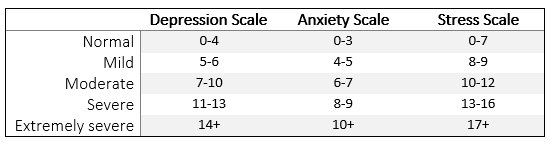
\includegraphics[width=0.8\linewidth]{images/DASS_Scoring} 

}

\caption{Classifications for DASS scores.}\label{fig:Figure8-1}
\end{figure}

\textbf{Formats}

You can download the DASS-21 as a PDF from the official \href{http://www2.psy.unsw.edu.au/groups/dass/}{DASS Homepage} or as a Qualtrics file below.

\href{questionnaires/DASS-21.qsf}{Qualtrics}

\textbf{Source:}

Lovibond, S.H. \& Lovibond, P.F. (1995). \emph{Manual for the Depression Anxiety Stress Scales.} (2nd. Ed.) Sydney: Psychology Foundation.

\hypertarget{modified-abbreviated-math-anxiety-scale}{%
\subsection{(Modified) Abbreviated Math Anxiety Scale}\label{modified-abbreviated-math-anxiety-scale}}

The Modified Abbreviated Math Anxiety Scale (mAMAS) was developed by Carey, Hill, Devine, and Szűcs (2017) and is based on the Abbreviated Math Anxiety Scale (AMAS) which was developed by Hopko, Mahadevan, Bare, and Hunt (2003). The wording of both scales is slightly different and in parts reflects that the data used to assess the suitability of the AMAS was collected in the US and the data used to assess suitability of the mAMAS was collected in the UK. The mAMAS can also be used to test children (approx. 8-13 years) while the use of the AMAS was verified for older teenagers and young adults.

The overall score of the AMAS and mAMAS in indicative of math anxiety in general but both measures also provide an estimate of anxiety related to being tested on mathematical knowledge and anxiety related to studying mathematics.

\textbf{How to use the (m)AMAS}

Both the AMAS and the mAMAS contain 9 questions and answers are scored on a 5-point Likert scale. Math evaluation (test) anxiety is assessed by the combined score of the even questions (2, 4, 6, 8) and math learning anxiety is assessed by the total score of the odd questions (1, 3, 5, 7, 9).

\textbf{Formats}

The AMAS and mAMAS can be downloaded as Qualtrics and Word file:

\href{questionnaires/AbbreviatedMathAnxietyScale.qsf}{Qualtrics - AMAS}\textbar{}\href{questionnaires/AbbreviatedMathAnxietyScale.docx}{Word - AMAS}

\href{questionnaires/ModifiedAbbreviatedMathAnxietyScale.qsf}{Qualtrics - mAMAS}\textbar{}\href{questionnaires/ModifiedAbbreviatedMathAnxietyScale.docx}{Word - mAMAS}

\textbf{Source:}

Carey, E., Hill, F., Devine, A., \& Szűcs, D. (2017). \href{https://www.frontiersin.org/articles/10.3389/fpsyg.2017.00011/full}{The modified abbreviated math anxiety scale: A valid and reliable instrument for use with children.} \emph{Frontiers in Psychology, 8}, 11.

Hopko, D. R., Mahadevan, R., Bare, R. L., \& Hunt, M. K. (2003). \href{https://www.researchgate.net/profile/Stephen_Joy/post/Hello_Can_anyone_tell_me_how_to_access_the_Abbreviated_Math_Anxiety_Scale_developed_by_Derek_Hopko2/attachment/59d624eb79197b80779833c8/AS:315374518636545@1452202552608/download/Math+Anxiety+Scale+Abbreviated+2003.pdf}{The abbreviated math anxiety scale (AMAS) construction, validity, and reliability.} \emph{Assessment, 10(2)}, 178-182.

\hypertarget{autism}{%
\section{Autism}\label{autism}}

The Autism Spectrum Quotient 10 items (AQ-10) scale was developed as a quick way to decide whether further autism diagnostics should be conducted. There three versions of the AQ-10, one for children, one for adolescents, and one for adults.

\textbf{How to use the AQ-10}

\emph{Adult AQ-10:}

\begin{itemize}
\tightlist
\item
  For questions 1, 7, 8, and 10, award one point if the response was `Slightly Agree' or `Definitely Agree'.
\item
  For questions 2, 3, 4, 5, 6, and 9, award one point if the response was `Slightly Disagree' or `Definitely Disagree'.
\end{itemize}

\emph{Adolescent AQ-10:}

\begin{itemize}
\tightlist
\item
  For questions 1, 5, 8 and 10, award one point if the response was `Slightly Agree' or `Definitely Agree'.
\item
  For questions 2, 3, 4, 6, 7 and 9, award one point if the response was `Slightly Disagree' or `Definitely Disagree'.
\end{itemize}

\emph{Children AQ-10:}

\begin{itemize}
\tightlist
\item
  For questions 1, 5, 7 and 10, award one point if the response was `Slightly Agree' or `Definitely Agree'.
\item
  For questions 2, 3, 4, 6, 8 and 9, award one point if the response was `Slightly Disagree' or `Definitely Disagree'.
\end{itemize}

A score of 6 or more suggests autistic tendencies. In a clinical context, the person would be referred for further diagnostics.

\textbf{Formats}

Qualtrics and paper-based versions of the AQ-10 can be downloaded for children, adolescents, and adults below. Versions in alternative languages can be found \href{https://www.autismresearchcentre.com/arc_tests}{here}.

\href{questionnaires/AutismSpectrumQuotient_Adults.qsf}{Qualtrics-Adults}\textbar{}\href{questionnaires/AutismSpectrumQuotient_Adolescent.qsf}{Qualtrics-Adolescents}\textbar{}\href{questionnaires/AutismSpectrumQuotient_Children.qsf}{Qualtrics-Children}

\href{questionnaires/AutismSpectrumQuotient_Adults.docx}{Word-Adults}\textbar{}\href{questionnaires/AutismSpectrumQuotient_Adolescent.docx}{Word-Adolescents}\textbar{}\href{questionnaires/AutismSpectrumQuotient_Children.docx}{Word-Children}

\textbf{Source:}

Allison, C., Auyeung, B., \& Baron-Cohen, S. (2012). \href{http://citeseerx.ist.psu.edu/viewdoc/download?doi=10.1.1.232.4537\&rep=rep1\&type=pdf}{Toward Brief ``Red Flags'' for Autism Screening: The Short Autism Spectrum Quotient and the Short Quantitative Checklist in 1,000 Cases and 3,000 Controls.} \emph{Journal of the American Acad of Child \& Adolescent Psychiatry, 51}(2), 202-212.

\hypertarget{internet-and-social-media-related}{%
\section{Internet and Social Media related}\label{internet-and-social-media-related}}

\hypertarget{problematic-internet-use-questionnaire-piuq}{%
\subsection{Problematic Internet Use Questionnaire (PIUQ)}\label{problematic-internet-use-questionnaire-piuq}}

The PIUQ was developed by Demetrovics,Szeredi, and Rózsa (2008). It assesses problematic internet use on three subscales: Obsession, Neglect, and Control Disorder. In other words, it provides an indication of how obsessed someone is with using the internet, to what degree this leads them to neglect other responsibilities, and whether they are in control of their behaviour. Each subscale contains five questions.

\textbf{How to use the PIUQ}

The PIUQ uses means related to each subscale. The mean score for each subscale can range from 6 to 30. When you analyse the data for each participant, you simply calculate their mean score for each subscale.

\textbf{Formats}

You can download the PIUQ as a Microsoft Word or as a Qualtrics file.

\href{questionnaires/ProblematicInternetUseQuestionnaire.qsf}{Qualtrics} \textbar{}
\href{questionnaires/ProblematicInternetUseQuestionnaire.docx}{Word}

\textbf{Source:}

Demetrovics, Z., Szeredi, B., \& Rózsa, S. (2008). \href{https://link.springer.com/content/pdf/10.3758/BRM.40.2.563}{The three-factor model of Internet addiction: The development of the Problematic Internet Use Questionnaire.} \emph{Behavior Research Methods, 40}, 563-574.

\hypertarget{general-mental-health}{%
\section{General Mental Health}\label{general-mental-health}}

The Mental Health Continuum - Short Form (MHC-SF) was developed by Keyes (2002) and measures general mental health in relation to emotional wellbeing, social wellbeing, and psychological wellbeing.Two versions of the MHC-SF exist, one for adults (18 years and older) and one for teenagers (12-18 years).

\textbf{How to use the MHC-SF}

The both MHC-SF versions contain 14 items and require participants to rate how often they experienced a feeling within the last month.

\emph{The rating scale is:}

0 = never

1 = once or twice

2 = about once a week

3 = about 2 to 3 times a week

4 = almost every day

5 = every day

Items 1-3 are linked to emotional wellbeing, Items 4-8 are linked to social wellbeing, and items 9 to 14 are linked to psychological wellbeing.

People are classified as `flourishing' or `languishing' based on their responses.

\textbf{Formats}

You can download the MHC-SF as a Microsoft Word or as a Qualtrics file.

\href{questionnaires/MentalHealthContinuum_Adults.qsf}{Qualtrics} \textbar{}
\href{questionnaires/MentalHealthContinuum_Adults.docx}{Word}

\textbf{Source:}

Keyes, C. L. (2002). \href{https://www.researchgate.net/profile/Corey_Keyes/publication/11278728_The_Mental_Health_Continuum_From_Languishing_to_Flourishing_in_Life/links/0046352b1a6f89da77000000/The-Mental-Health-Continuum-From-Languishing-to-Flourishing-in-Life.pdf}{The mental health continuum: From languishing to flourishing in life.} \emph{Journal of Health and Social Behavior,} 207-222.

Keyes, C. L. (2009). \href{https://www.aacu.org/sites/default/files/MHC-SFEnglish.pdf}{Brief description of the mental health continuum short form (MHC-SF).}

\hypertarget{qualtrics}{%
\chapter{Qualtrics}\label{qualtrics}}

Qualtrics is an online tool that can be used to run surveys. If you want to use Qualtrics, you need to register through the University of Strathclyde. You can do this by clicking \href{https://www.strath.ac.uk/is/software/qualtrics/}{here}. The information under ``How do I get it?'' tells you what to do to register through the university.

\hypertarget{how-to-import-questionnaires-into-qualtrics}{%
\section{How to import questionnaires into Qualtrics}\label{how-to-import-questionnaires-into-qualtrics}}

For most questionnaires, you will have the option to download a Qualtrics file.

\begin{enumerate}
\def\labelenumi{\arabic{enumi}.}
\tightlist
\item
  Choose a survey and download the Qualtrics file to your computer.
\item
  Log on to Qualtrics through the University of Strathclyde link.
\item
  Find the ``Create New Project'' option. In some cases, you may need to click on ``Projects'' in the menu at the top first.
\end{enumerate}

\begin{figure}

{\centering 
\includegraphics[width=0.85\linewidth]{images/Qualtrics/02NewProject} 

}

\caption{Click on "Create new Project" - you may need to click on "Projects" first to get the option.}\label{fig:Figure11-2}
\end{figure}

This will take you here:

\begin{figure}

{\centering 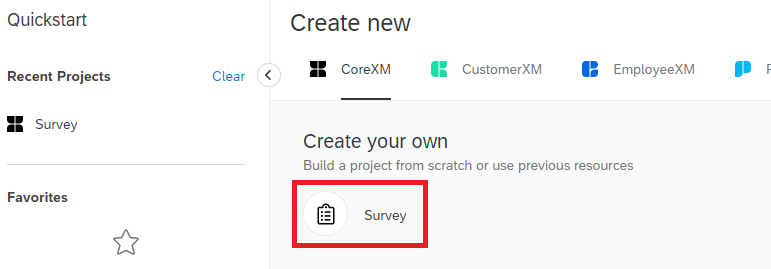
\includegraphics[width=0.85\linewidth]{images/Qualtrics/03NewProject2} 

}

\caption{Click on "Survey", framed in red.}\label{fig:Figure11-3}
\end{figure}

\begin{enumerate}
\def\labelenumi{\arabic{enumi}.}
\setcounter{enumi}{3}
\tightlist
\item
  Click on ``Survey'', which is framed in red in the picture above. This will show you the following options, for which you should choose ``From a File''
\end{enumerate}

\begin{figure}

{\centering 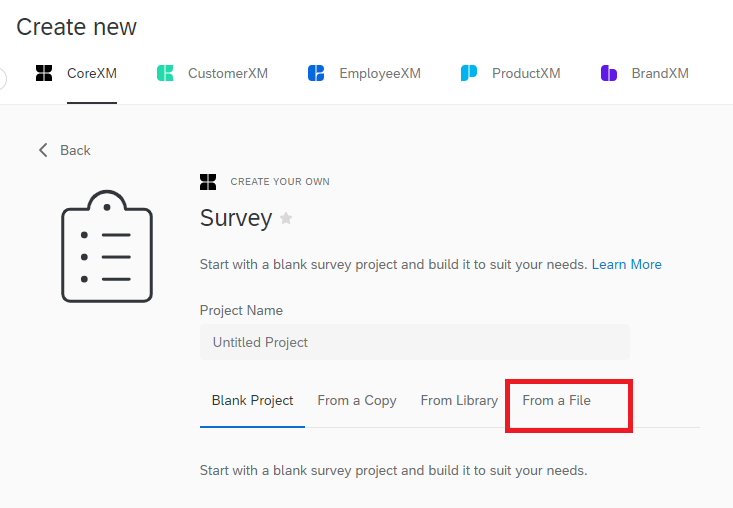
\includegraphics[width=0.85\linewidth]{images/Qualtrics/04FromFile} 

}

\caption{Choose "From a File" to upload the experiment file you downloaded earlier.}\label{fig:Figure11-4}
\end{figure}

\begin{enumerate}
\def\labelenumi{\arabic{enumi}.}
\setcounter{enumi}{4}
\tightlist
\item
  The file will not be uploaded automatically. First, you have a chance to change the project name and check that you have chosen the right file. The default project name is the file name. For this example, we are going to change it to ``PIUQ''. Then, click ``Get Started''
\end{enumerate}

\begin{figure}

{\centering 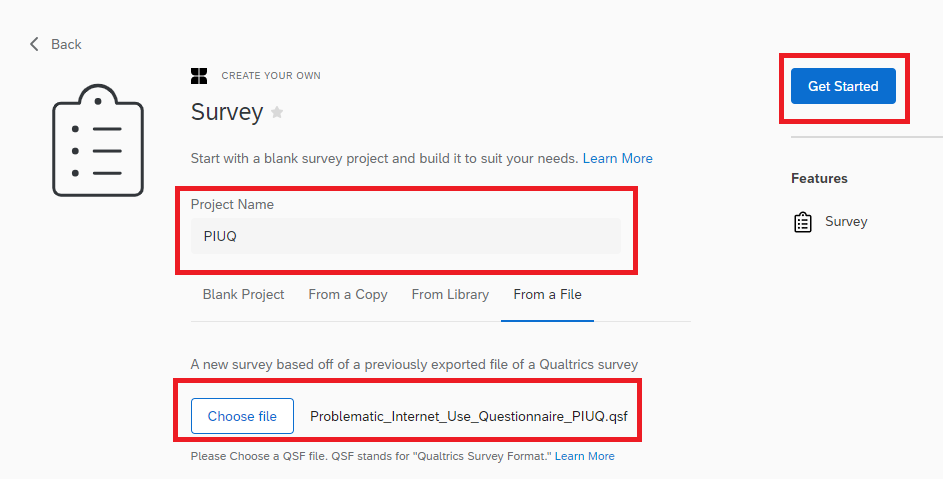
\includegraphics[width=0.85\linewidth]{images/Qualtrics/05FromFile2} 

}

\caption{Check that you have chosen the correct file and re-name the survey, if you want to.}\label{fig:Figure11-5}
\end{figure}

\begin{enumerate}
\def\labelenumi{\arabic{enumi}.}
\setcounter{enumi}{5}
\tightlist
\item
  The next screen will show you the imported questions. Check that they match the questions and responses you can find in the Word file of the survey.
\end{enumerate}

\begin{figure}

{\centering 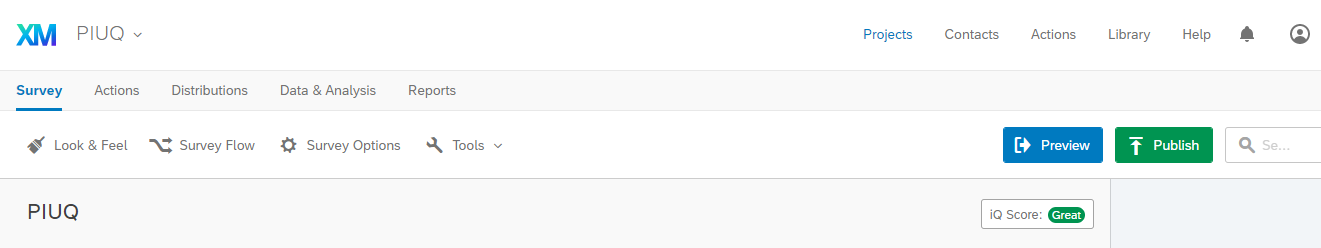
\includegraphics[width=0.85\linewidth]{images/Qualtrics/07Done} 

}

\caption{Make sure the answers were imported correctly.}\label{fig:Figure11-6}
\end{figure}

If you click on ``Projects'' in the main menu, it will take you to an overview of the surveys you currently have uploaded.

\hypertarget{how-to-test-data-recording}{%
\section{How to test data recording}\label{how-to-test-data-recording}}

\hypertarget{generate-pilot-data}{%
\subsection{Generate pilot data}\label{generate-pilot-data}}

It is a good idea to test if your survey records the answers the way it is supposed to. To do this, you have two options:

\textbf{Option 1:} Click on Preview and answer the survey questions yourself. When the survey is finished, it will record your responses as it would also for a real participant.

\begin{figure}

{\centering 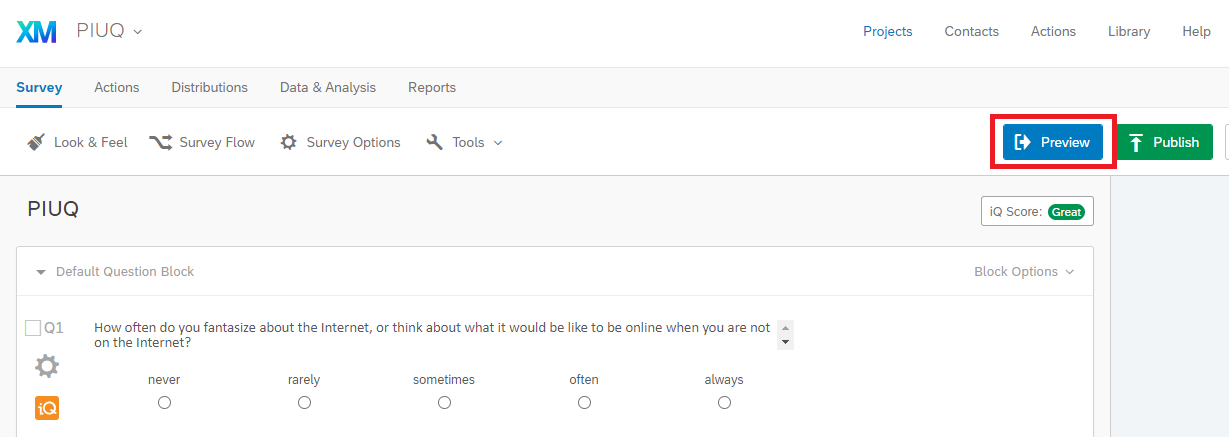
\includegraphics[width=0.85\linewidth]{images/Qualtrics/08Preview} 

}

\caption{Click on Preview to see what the questions look like online and on a phone.}\label{fig:Figure11-7}
\end{figure}

\textbf{Option 2:} Let Qualtrics generate some test responses.To do this, open your survey and choose ``Tools'' -\textgreater{} ``Review'' -\textgreater{} ``Generate Test Responses\ldots{}''

\begin{figure}

{\centering 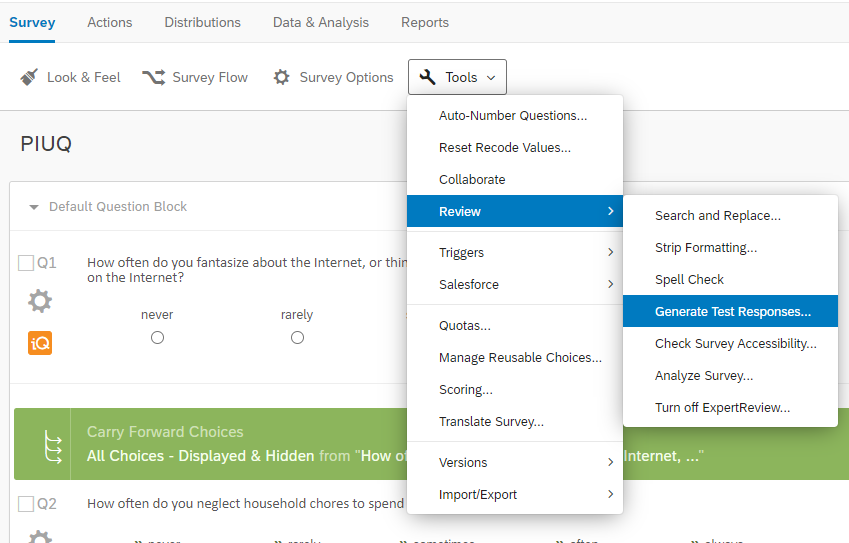
\includegraphics[width=0.85\linewidth]{images/Qualtrics/09testresponses1} 

}

\caption{Choose "Tools" -> "Review" -> "Generate Test Responses...".}\label{fig:Figure11-8}
\end{figure}

This will lead you here:

\begin{figure}

{\centering 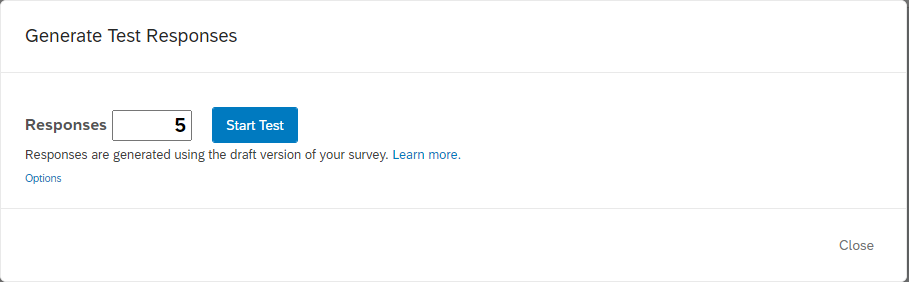
\includegraphics[width=0.85\linewidth]{images/Qualtrics/10testresponses2} 

}

\caption{By changing the number of responses, you can adjust how many test "participants" you want Qualtrics to generate.}\label{fig:Figure11-9}
\end{figure}

The number of ``Responses'' represents the number of participants, e.g.~if you tell Qualtrics to generate five responses, it will create test data that looks as if five participants have responded. When you are ready, click on ``Start Test.''

If everything went well, you should see something like this:

\begin{figure}

{\centering 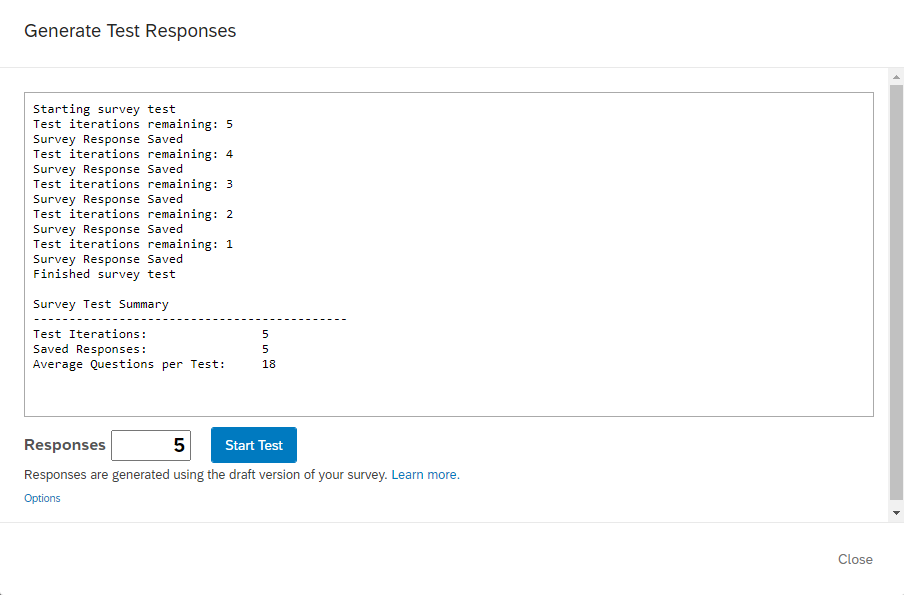
\includegraphics[width=0.85\linewidth]{images/Qualtrics/11testresponses3} 

}

\caption{Output after the test data has been generated.}\label{fig:Figure11-10}
\end{figure}

The data has now been generated and you can click ``Close''

\hypertarget{check-pilot-data}{%
\subsection{Check pilot data}\label{check-pilot-data}}

We can access the data by clicking on ``Data and Analysis'':

\begin{figure}

{\centering 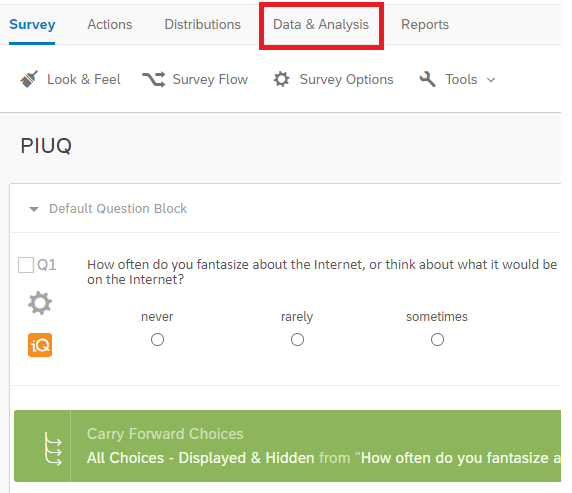
\includegraphics[width=0.85\linewidth]{images/Qualtrics/12checkdata1} 

}

\caption{To access the data collected with your survey, click on "Data and Analysis"}\label{fig:Figure11-11}
\end{figure}

Usually, your data will be shown after clicking on the tab. However, if you have only recently created the test data, it may take a little while to appear. Similarly, when your survey is online and many participants responded right before you check the data, it may take some time to update this section. In that case, you might not see data here but a message that tells you that responses are being re-indexed:

\begin{figure}

{\centering 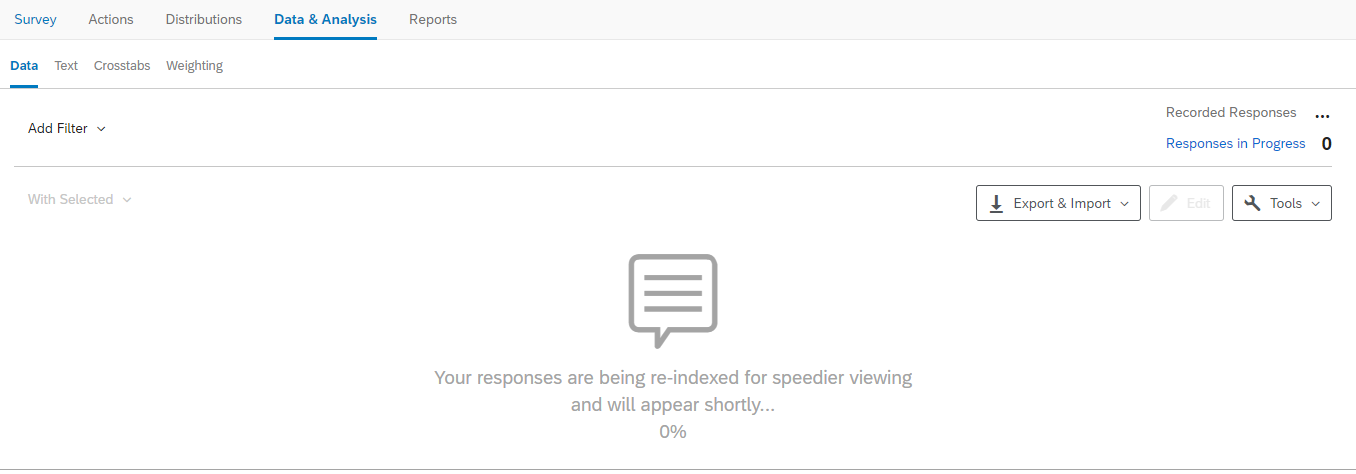
\includegraphics[width=0.85\linewidth]{images/Qualtrics/13checkdata2} 

}

\caption{To access the data collected with your survey, click on "Data and Analysis"}\label{fig:Figure11-12}
\end{figure}

Usually, this message should disappear after about 10 to 30 minutes. However, occasionally, it may take a little longer. If you cannot see the data after 24h, get in touch with the Qualtrics support team. Very rarely, the automatic re-indexing runs into an issue and their support team will be able to rectify this issue. Your data will \textbf{not} be lost if this happens.

After responses are re-indexed, the data tab should look like this:

\begin{figure}

{\centering 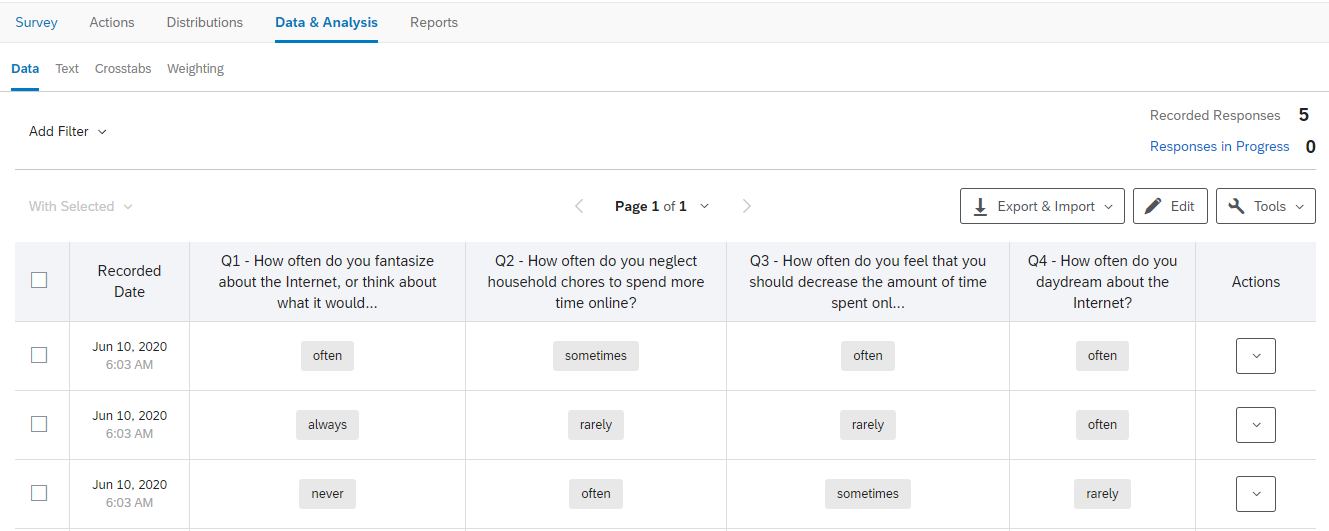
\includegraphics[width=0.99\linewidth]{images/Qualtrics/13checkdata3} 

}

\caption{Data overview in "Data and Analysis"}\label{fig:Figure11-13}
\end{figure}

To analyse the data, and to check if responses are exported correctly, click on ``Export \& Import'' and then ``Export data\ldots{}''

\begin{figure}

{\centering 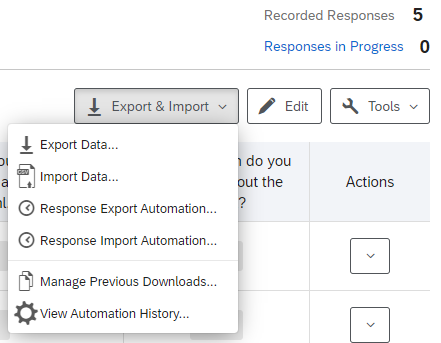
\includegraphics[width=0.85\linewidth]{images/Qualtrics/14exportdata} 

}

\caption{Choose "Export and Import" -> "Export data..." to dowload your data.}\label{fig:Figure11-14}
\end{figure}

This will take you here:

\begin{figure}

{\centering 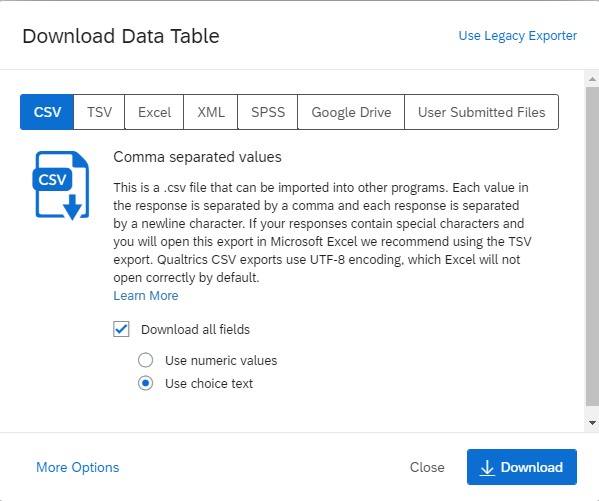
\includegraphics[width=0.85\linewidth]{images/Qualtrics/15exportdata} 

}

\caption{You can choose from a range of output format, e.g. Excel, SPSS.}\label{fig:Figure11-15}
\end{figure}

Just choose the format in which you would like to download your data.

\hypertarget{scoring}{%
\section{Scoring}\label{scoring}}

Unfortunately, exporting and then importing a study tends to remove scoring information from the Qualtrics file.

The Qualtrics guide on how to set up scoring can be found \href{https://www.qualtrics.com/support/survey-platform/survey-module/survey-tools/scoring/}{here}. Using scoring means you can tell Qualtrics which questions to score in reverse and which questions it should use to calculate a subscore.

If you don't want to use scoring, you can calculate scores in SPSS later.

\hypertarget{importing-questions-only}{%
\section{Importing Questions only}\label{importing-questions-only}}

To import one of the prepared questionnaires, open the survey you want to add them to and click on `Import Questions from.'

\begin{figure}

{\centering \includegraphics[width=0.85\linewidth]{images/Qualtrics/import} 

}

\caption{Click on Import Questions from}\label{fig:Figure11-16}
\end{figure}

In the next window click on \textbf{`My Surveys'} and then choose the survey that contains the question you are interested in. If the survey is a file you have downloaded from here, you can just add the whole survey, as each file only contains one question.

\hypertarget{open-sesame}{%
\chapter{Open Sesame}\label{open-sesame}}

Open Sesame is a program that allows you to run experiments on a computer, tablet, or online. Most experiments included in this Experiment Library will be set up in Open Sesame, while questionnaires will be prepared for Qualtrics.

\hypertarget{how-to-install-open-sesame}{%
\section{How to install Open Sesame}\label{how-to-install-open-sesame}}

The experiments included in this Experiment Library were programmed in \textbf{Open Sesame 3.3.2} To avoid problems when executing the experiments, please install the same version.

\hypertarget{windows}{%
\subsection{Windows:}\label{windows}}

\begin{enumerate}
\def\labelenumi{\arabic{enumi}.}
\tightlist
\item
  There are two ways in which you can install Open Sesame.

  \begin{itemize}
  \tightlist
  \item
    \textbf{Option 1:} Download the program file and install Open Sesame. To choose this option, download the file that is appropriate for your Windows system: \href{https://github.com/open-cogsci/OpenSesame/releases/download/release\%2F3.3.2/opensesame_3.3.2-py27-win64-1.exe}{click here}
  \item
    \textbf{Option 2:} Download a zip-folder with all the required files. If you choose this option, you need to unzip the file and double-click \emph{``opensesame''} everytime you want to use Open Sesame. This is less convenient but can be a good option if you cannot install new software (e.g.~because of IT restrictions) or want to use different versions of Open Sesame in parallel.If you prefer this option : \href{https://github.com/open-cogsci/OpenSesame/releases/download/release\%2F3.3.2/opensesame_3.3.2-py27-win64-1.zip}{click here}.
  \end{itemize}
\item
  If you chose \textbf{Option 1}, double-click on the .exe file you have downloaded and follow the installation instructions. If you chose \textbf{Option 2}, unzip the folder you have downloaded. This usually takes a few minutes. Locate the \emph{``opensesame''} file and double-click on it - the programme should now open. Figure 11.1. shows a screenshot of the contents
\end{enumerate}

\begin{figure}

{\centering 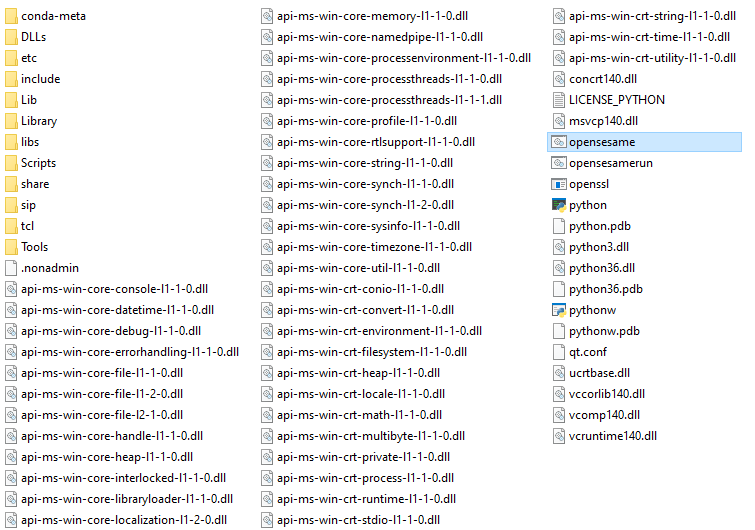
\includegraphics[width=0.85\linewidth]{images/opensesame/Option2} 

}

\caption{If you choose to dowload the zipped version of Open Sesame (Option 2), this is what you will see when you unzip the folder. Double-click on the "opensesame" file to start the program.}\label{fig:Figure12-1}
\end{figure}

\begin{enumerate}
\def\labelenumi{\arabic{enumi}.}
\setcounter{enumi}{2}
\tightlist
\item
  Check if the program opens without issues.
\end{enumerate}

\hypertarget{mac-os}{%
\subsection{Mac OS}\label{mac-os}}

If you use a Mac computer, you can download Open Sesame from here:
\href{https://github.com/open-cogsci/OpenSesame/releases/download/release\%2F3.3.2/opensesame_3.3.2-py37-macos-1.dmg}{Mac OS}

In some cases, Open Sesame may be prevented from installing/launching. If you run into this issue, please follow \href{https://support.apple.com/en-in/guide/mac-help/mh40616/mac}{Apple's advice} on how to work around this problem.

\hypertarget{open-sesame-tutorials}{%
\section{Open Sesame Tutorials}\label{open-sesame-tutorials}}

The \href{osdoc.cogsci.nl}{official Open Sesame homepage} has a wide range of tutorials that allow you to learn how to use it. The one I would recommend to start with is the \href{https://osdoc.cogsci.nl/3.3/tutorials/beginner/}{beginners gaze cueing paradigm}.

\hypertarget{open-sesame-the-basics}{%
\section{Open Sesame: The Basics}\label{open-sesame-the-basics}}

When you open Open Sesame for the first time, it will look like this.

\begin{figure}

{\centering 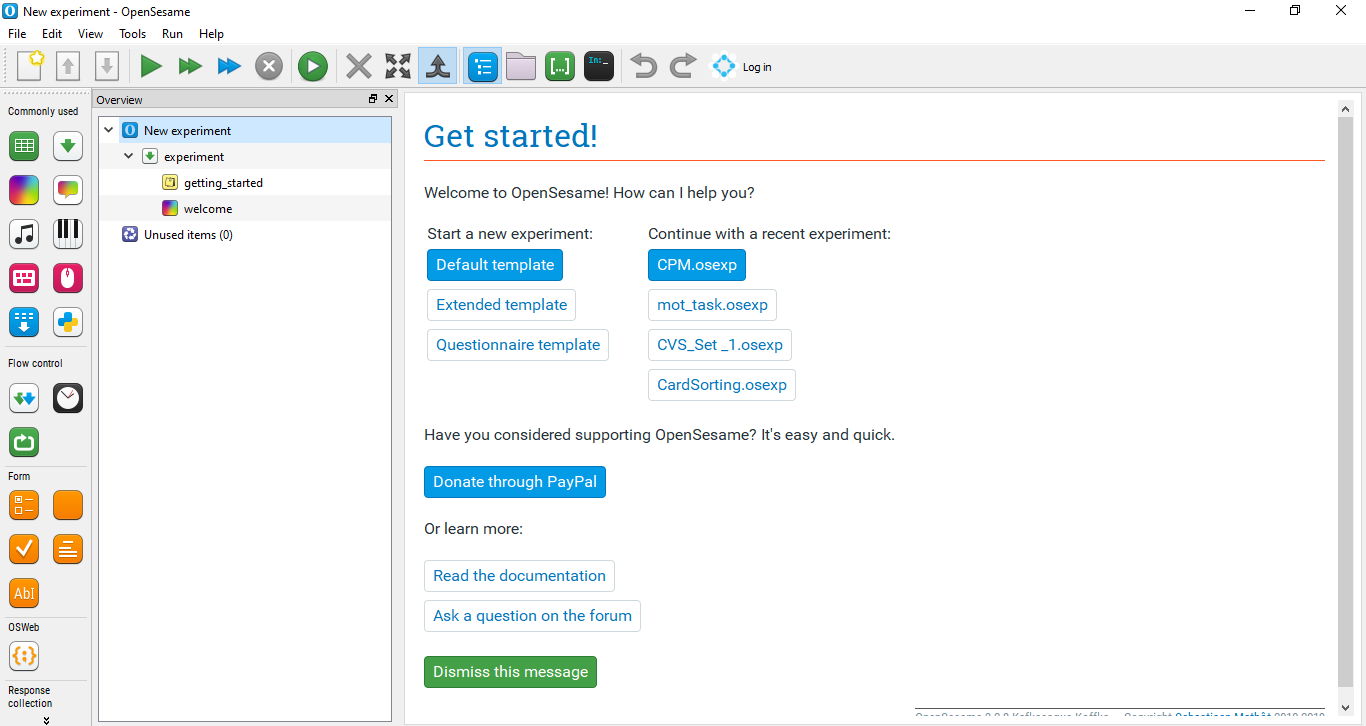
\includegraphics[width=0.85\linewidth]{images/opensesame/OpenSesameopen} 

}

\caption{This is what Open Sesame looks like when you open it.}\label{fig:Figure12-2}
\end{figure}

So what are all of these buttons? Have a look around. When you hover over buttons, Open Sesame will tell you what they are good for.

\begin{figure}

{\centering 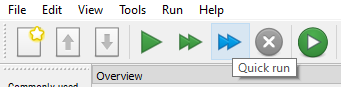
\includegraphics[width=0.85\linewidth]{images/opensesame/hover} 

}

\caption{If you hover over buttons, Open Sesame will tell you their function.}\label{fig:Figure12-3}
\end{figure}

To run an experiment, you have four options. Use ``Run fullscreen'' to test participants on a computer. Choose Quickrun or ``Run in Window'' to test if the experiment runs smoothly and all variables are recorded.'Run in browser' can be used to check if the experiments is suitable to run online.

\begin{figure}

{\centering 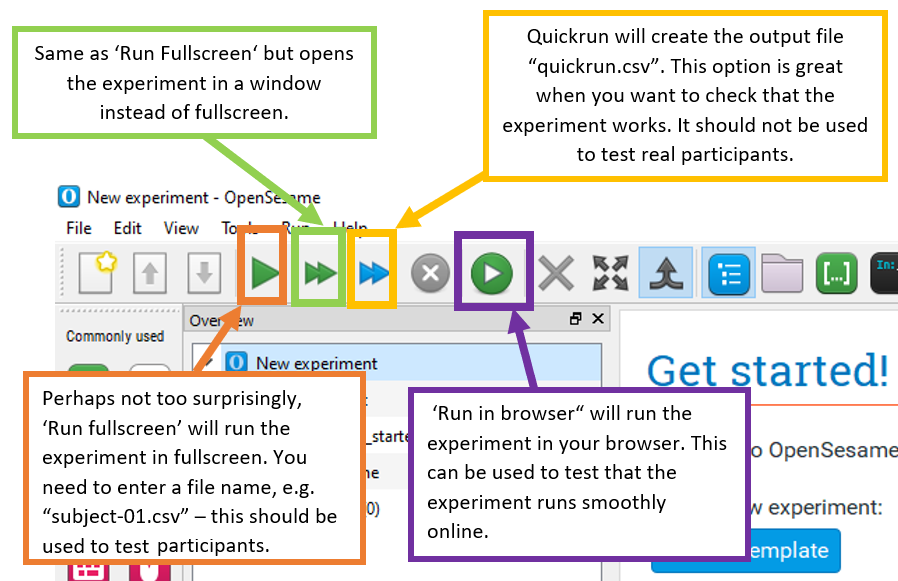
\includegraphics[width=0.85\linewidth]{images/opensesame/runexp} 

}

\caption{Choose the option that suits your needs best.}\label{fig:Figure12-4}
\end{figure}

If you have already downloaded one of the experiments, you can open it now and give it a try. If you have not decided on a experiment yet, Open Sesame comes with a small number of pre-installed experiments you can find by clicking on `Tools' and choosing `Example Experiments'

\hypertarget{starting-to-work-with-open-sesame}{%
\section{Starting to work with Open Sesame}\label{starting-to-work-with-open-sesame}}

If you choose one of the Open Sesame experiments, you may want to add a question or combine tasks. We will have a look at how to add some simple questions and how to combine tasks.

Start by downloading the two (or more) files you want to combine. Open both by \textbf{double-clicking} on the files, so they open in two seperate windows. To copy elements from one experiment to another, right-click on the element you want to copy and choose `copy'. To paste it, right-click in the location you want to copy it to and choose `paste'

\hypertarget{loggers}{%
\section{Loggers}\label{loggers}}

Open Sesame experiments should only have one Logger element in each experiment file. If you combine experiments, delete one type of logger and replace it with the other. You can do this by choosing `copy (linked)' when you copy the logger. Then just paste it to the relevant locations.

\hypertarget{open-sesame-on-android}{%
\section{Open sesame on Android}\label{open-sesame-on-android}}

\textbf{Important information for the Android version}

If you want to run an \textbf{Android version} of a task, it should only be used on tablets and not on mobile phones - unless you yourself programmed it to be used on phones. The Android app allows you to run Open Sesame on a tablet but you cannot make any changes to the experiment file. This needs to happen on a computer. Importantly, the app you will need to download is no longer developed and you may thus experience issues if you are trying to develop a new experiment in the latest Open Sesame version. To avoid these issues, \textbf{please use Open Sesame version 3.1.8.}

To download the app, search for ``OpenSesame experiment runtime'' in the app store or \href{https://play.google.com/store/apps/details?id=nl.cogsci.opensesame}{click here}.

If you have a Windows computer, please check whether you have a 32-bit system or 64-bit system version of Windows installed. To find out how to do this, \href{https://www.howtogeek.com/howto/21726/how-do-i-know-if-im-running-32-bit-or-64-bit-windows-answers/}{click here}.

The download options for this Open Sesame version are to install it (and thus replace any other version you have installed) or download it as a Zip-file that does not require installation. Instructions on how to run Open Sesame from a Zip-file are provided in the Open Sesame Chapter. Download links for version 3.1.8 are below:

Install Windows:
\href{https://github.com/smathot/OpenSesame/releases/download/release\%2F3.1.8/opensesame_3.1.8-py3.5-win64-1.exe}{64-bit}
\href{https://github.com/smathot/OpenSesame/releases/download/release\%2F3.1.8/opensesame_3.1.8-py2.7-win32-1.exe}{32-bit}

Install on Mac OS: \href{https://github.com/smathot/OpenSesame/releases/download/release\%2F3.1.8/opensesame_3.1.8-py2.7-macos-1.dmg}{click here}

Download zipped folder for Windows:
\href{https://github.com/smathot/OpenSesame/releases/download/release\%2F3.1.8/opensesame_3.1.8-py3.5-win64-1.zip}{64-bit}
\href{https://github.com/smathot/OpenSesame/releases/download/release\%2F3.1.8/opensesame_3.1.8-py2.7-win32-1.zip}{32-bit}

\textbf{If you are downloading 3.1.8 as a Zip-File}

The file you need to execute in order to start Open Sesame is in a different location in this version of Open Sesame. Unzip the folder and open it. You will see a folder named \textbf{``Scripts''}. Open it and double-click \textbf{``opensesame''} to open Open Sesame. If you choose ``Android'' as a backend for your task, you can still develop new experiments for Android.

\hypertarget{open-sesame---online}{%
\chapter{Open Sesame - Online}\label{open-sesame---online}}

The \href{https://osdoc.cogsci.nl/3.2/manual/osweb/}{official Open Sesame website} provides some information on how to test experiments that were designed for use online.

If you are at the University of Strathclyde, you will have access to the university's JATOS server. Students should contact their supervisor to find out how to access the server. Staff that would like to use the server but who have not received the user guide can contact \href{jennifer.mattschey@strath.ac.uk}{Dr Jennifer Mattschey}.

\hypertarget{fullscreen-vs.-browser-window}{%
\section{Fullscreen vs.~Browser Window}\label{fullscreen-vs.-browser-window}}

We can set the experiment to run in full screen at two different points of the process. First, when we export the Open Sesame experiment as a JATOS study. In the OSWeb tab (\textbf{`Tools' --\textgreater{} `OSWeb'}), there is the option to tick \textbf{`Make browser fullscreen'}

\begin{figure}

{\centering 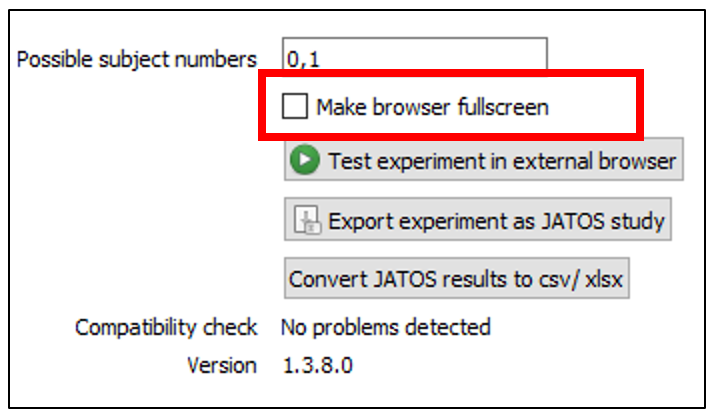
\includegraphics[width=0.5\linewidth]{images/opensesame/fullscreen1} 

}

\caption{Option 1 is to tick fullscreen when the experiment is exported as JATOS file.}\label{fig:Figure13-1}
\end{figure}

If the experiment is already uploaded and you want to change the presentation mode, go the uploaded experiment and click on \textbf{light blue component `Properties' button}, framed in red below.

\begin{figure}

{\centering 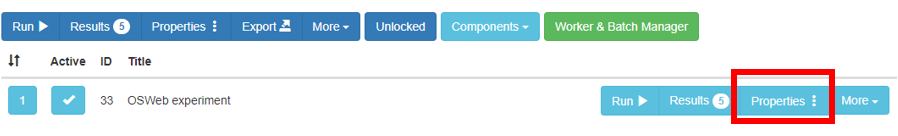
\includegraphics[width=0.99\linewidth]{images/opensesame/componentproperty} 

}

\caption{Option 1 is to tick fullscreen when the experiment is exported as JATOS file.}\label{fig:Figure13-2}
\end{figure}

This will open a window with the component properties. To change the presentation of the experiment to full screen, ``fullscreen'': false, needs to be changed to ``fullscreen'': true. After the change has been made and saved, the experiment will run in full screen.

\begin{figure}

{\centering 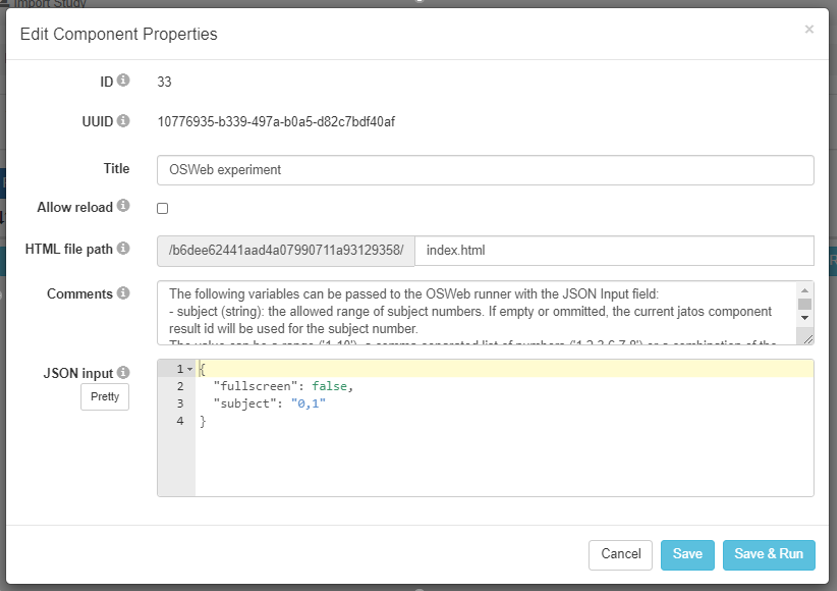
\includegraphics[width=0.99\linewidth]{images/opensesame/fullscreen2} 

}

\caption{Option 1 is to tick fullscreen when the experiment is exported as JATOS file.}\label{fig:Figure13-3}
\end{figure}

\hypertarget{sona}{%
\section{SONA}\label{sona}}

Using JATOS with SONA is possible but you will still need to mark participants as `participated' or `no show'. To do this, you need to find a way to identify them.

One way to achieve this is to download this file posted to the Open Sesame forum \href{https://forum.cogsci.nl/discussion/5876/}{by clicking here}. Just copy the file into your experiment file and remember to acknowledge its source. If you want to combine Qualtrics and Open Sesame, this also allows us to link both sets of data by asking participants to enter their participant ID.

\hypertarget{questionnaires}{%
\section{Questionnaires}\label{questionnaires}}

How can we add questionnaires if Open Sesame's form function can't be used online? One was is to think about the categories you want to include, e.g.~native vs non-native speakers of English. In that case, ``are you a native speaker of English? Press `Y' for yes and `N' for no'' paired with a keyboard response can provide sufficient information.

For more extensive questionnaires, using Qualtrics and Open Sesame could be an option. Ask participants to enter a participant ID to link the data (see \textbf{`SONA'} above). Finally, it is possible to add a javascript questionnaire as a separate component on the JATOS server. Information on how to do this will follow soon.

\end{document}
